\chapter{Experimental Data}
In order to validate the performance of the observer implementation, experimental data was collected with a Hokuyo UBG-04LX-F01 scanning laser range-finder.

Measurements were taken to:
\begin{itemize}
\item build a model of the noise characteristics of the Hokuyo UBG-04LX-F01 in order to more accurately simulate the performance of the observer;
\item observe the motion of a moving cube of known state to test the observer in real world conditions.
\end{itemize}

Section \ref{sensor_noise} details how measurements were taken - noise model 
Section \ref{testingdata} describes ongoing work. How data was collected, processed - how it can be used. 

\section{Sensor Noise Characterisation} \label{sensor_noise}
motivation - accurate noise model for simulation. In \cite{park2010characterization}, noise characterised but no unified model for range and angle. Furthermore, significant effect from surface colour, texture. Better to develop model for specific case - more accurate practical testing in the future.

	\subsection{Setup}
		\textbf{physical setup:} see \ref{fig:noise_setup}\\
		\textbf{error:} distance +/- 1mm, angle, +/- 0.5 degrees
		\textbf{measurement configurations:}\\
			-5cm increments from 0.25-1.75m\\
			-vary incidence angle: 0,20,40,60,80 degrees
		 
	\subsection{Results}
	Similar results to \cite{park2010characterization}. Difficult to get sensible readings at high angles, Gaussian distributed noise.
		\textbf{Error distribution:}
		Histograms (Figure \ref{fig:mean_hist}) - range error approximately normally distributed:
		\begin{figure}
		\centering
		  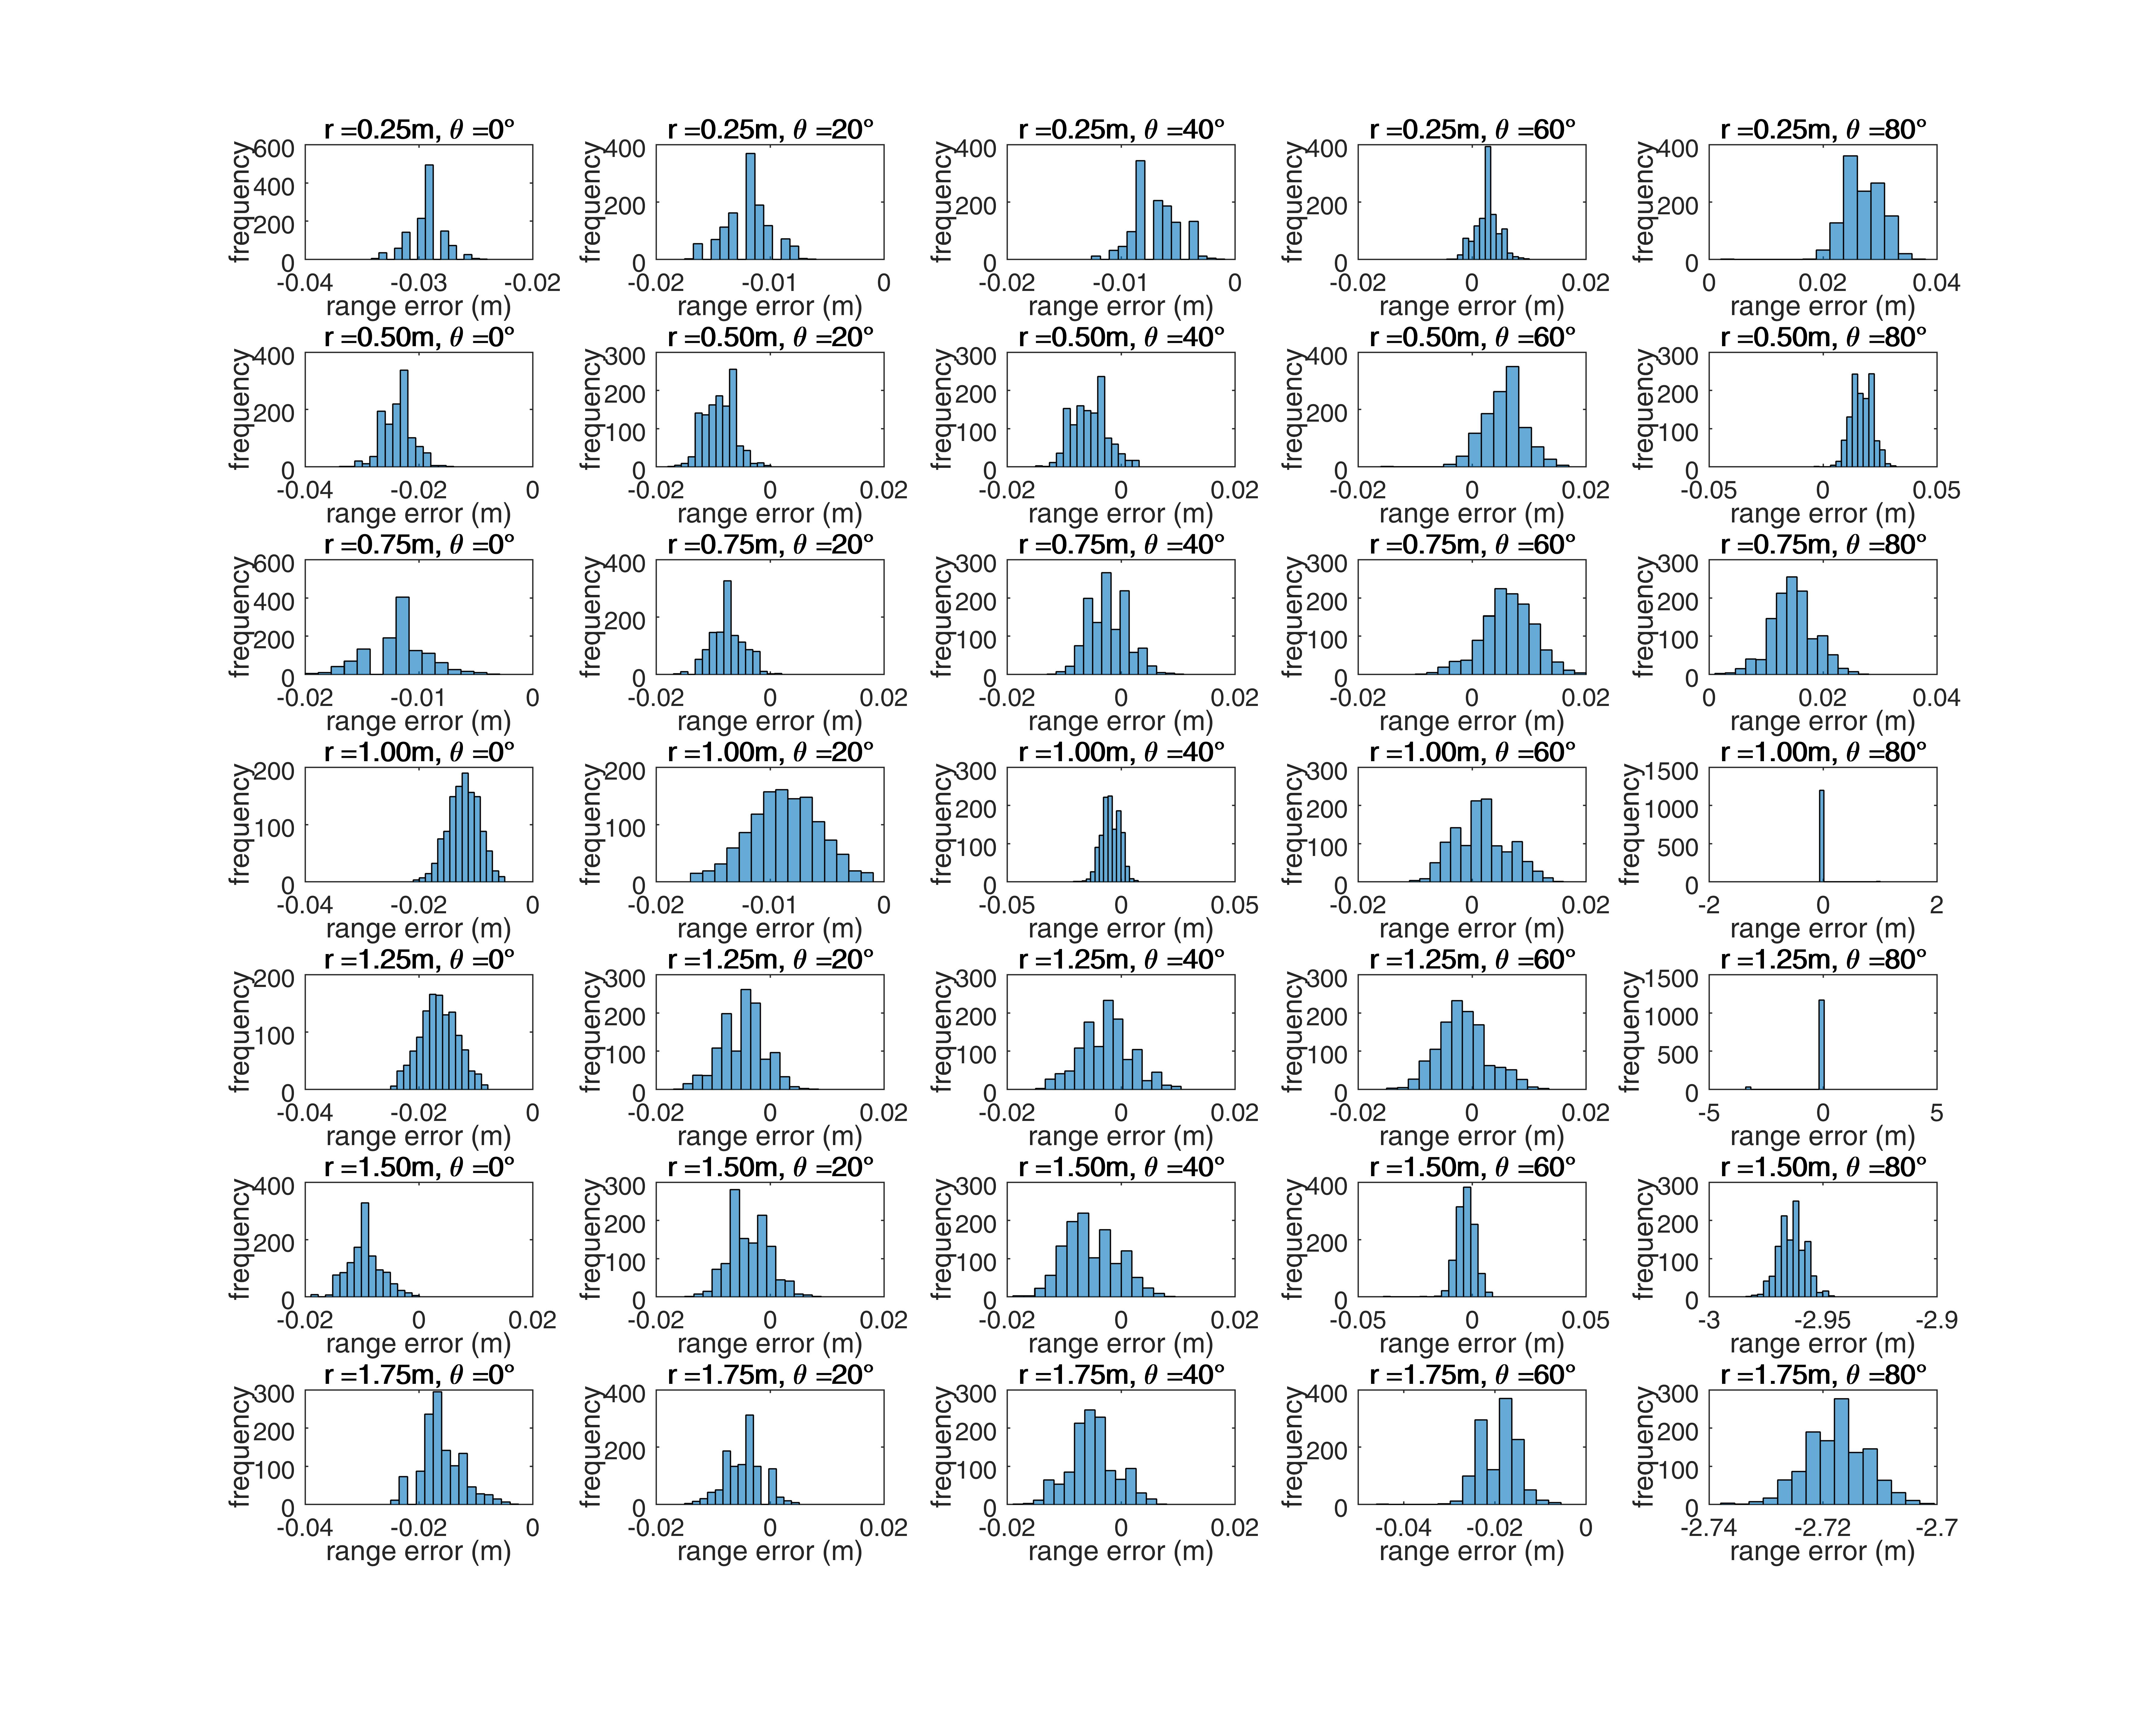
\includegraphics[width=1\textwidth,trim = 0mm 0mm 0mm 0mm,clip]{./Figures/range_error_histograms.jpg}
		  \caption{Sensor noise function $f_{UBG}(r,\theta)$ approximately normally distributed}
		  \label{fig:mean_hist}
		\end{figure}
		
		Mean range error as function of (range,incidence angle) - Figure \ref{fig:mean_range_error}
		\begin{figure}
	  		\centering
	  		\subfigure[\label{fig:mean_range_error_outliers}]{
	  		\begin{minipage}[b]{0.45\columnwidth}
    			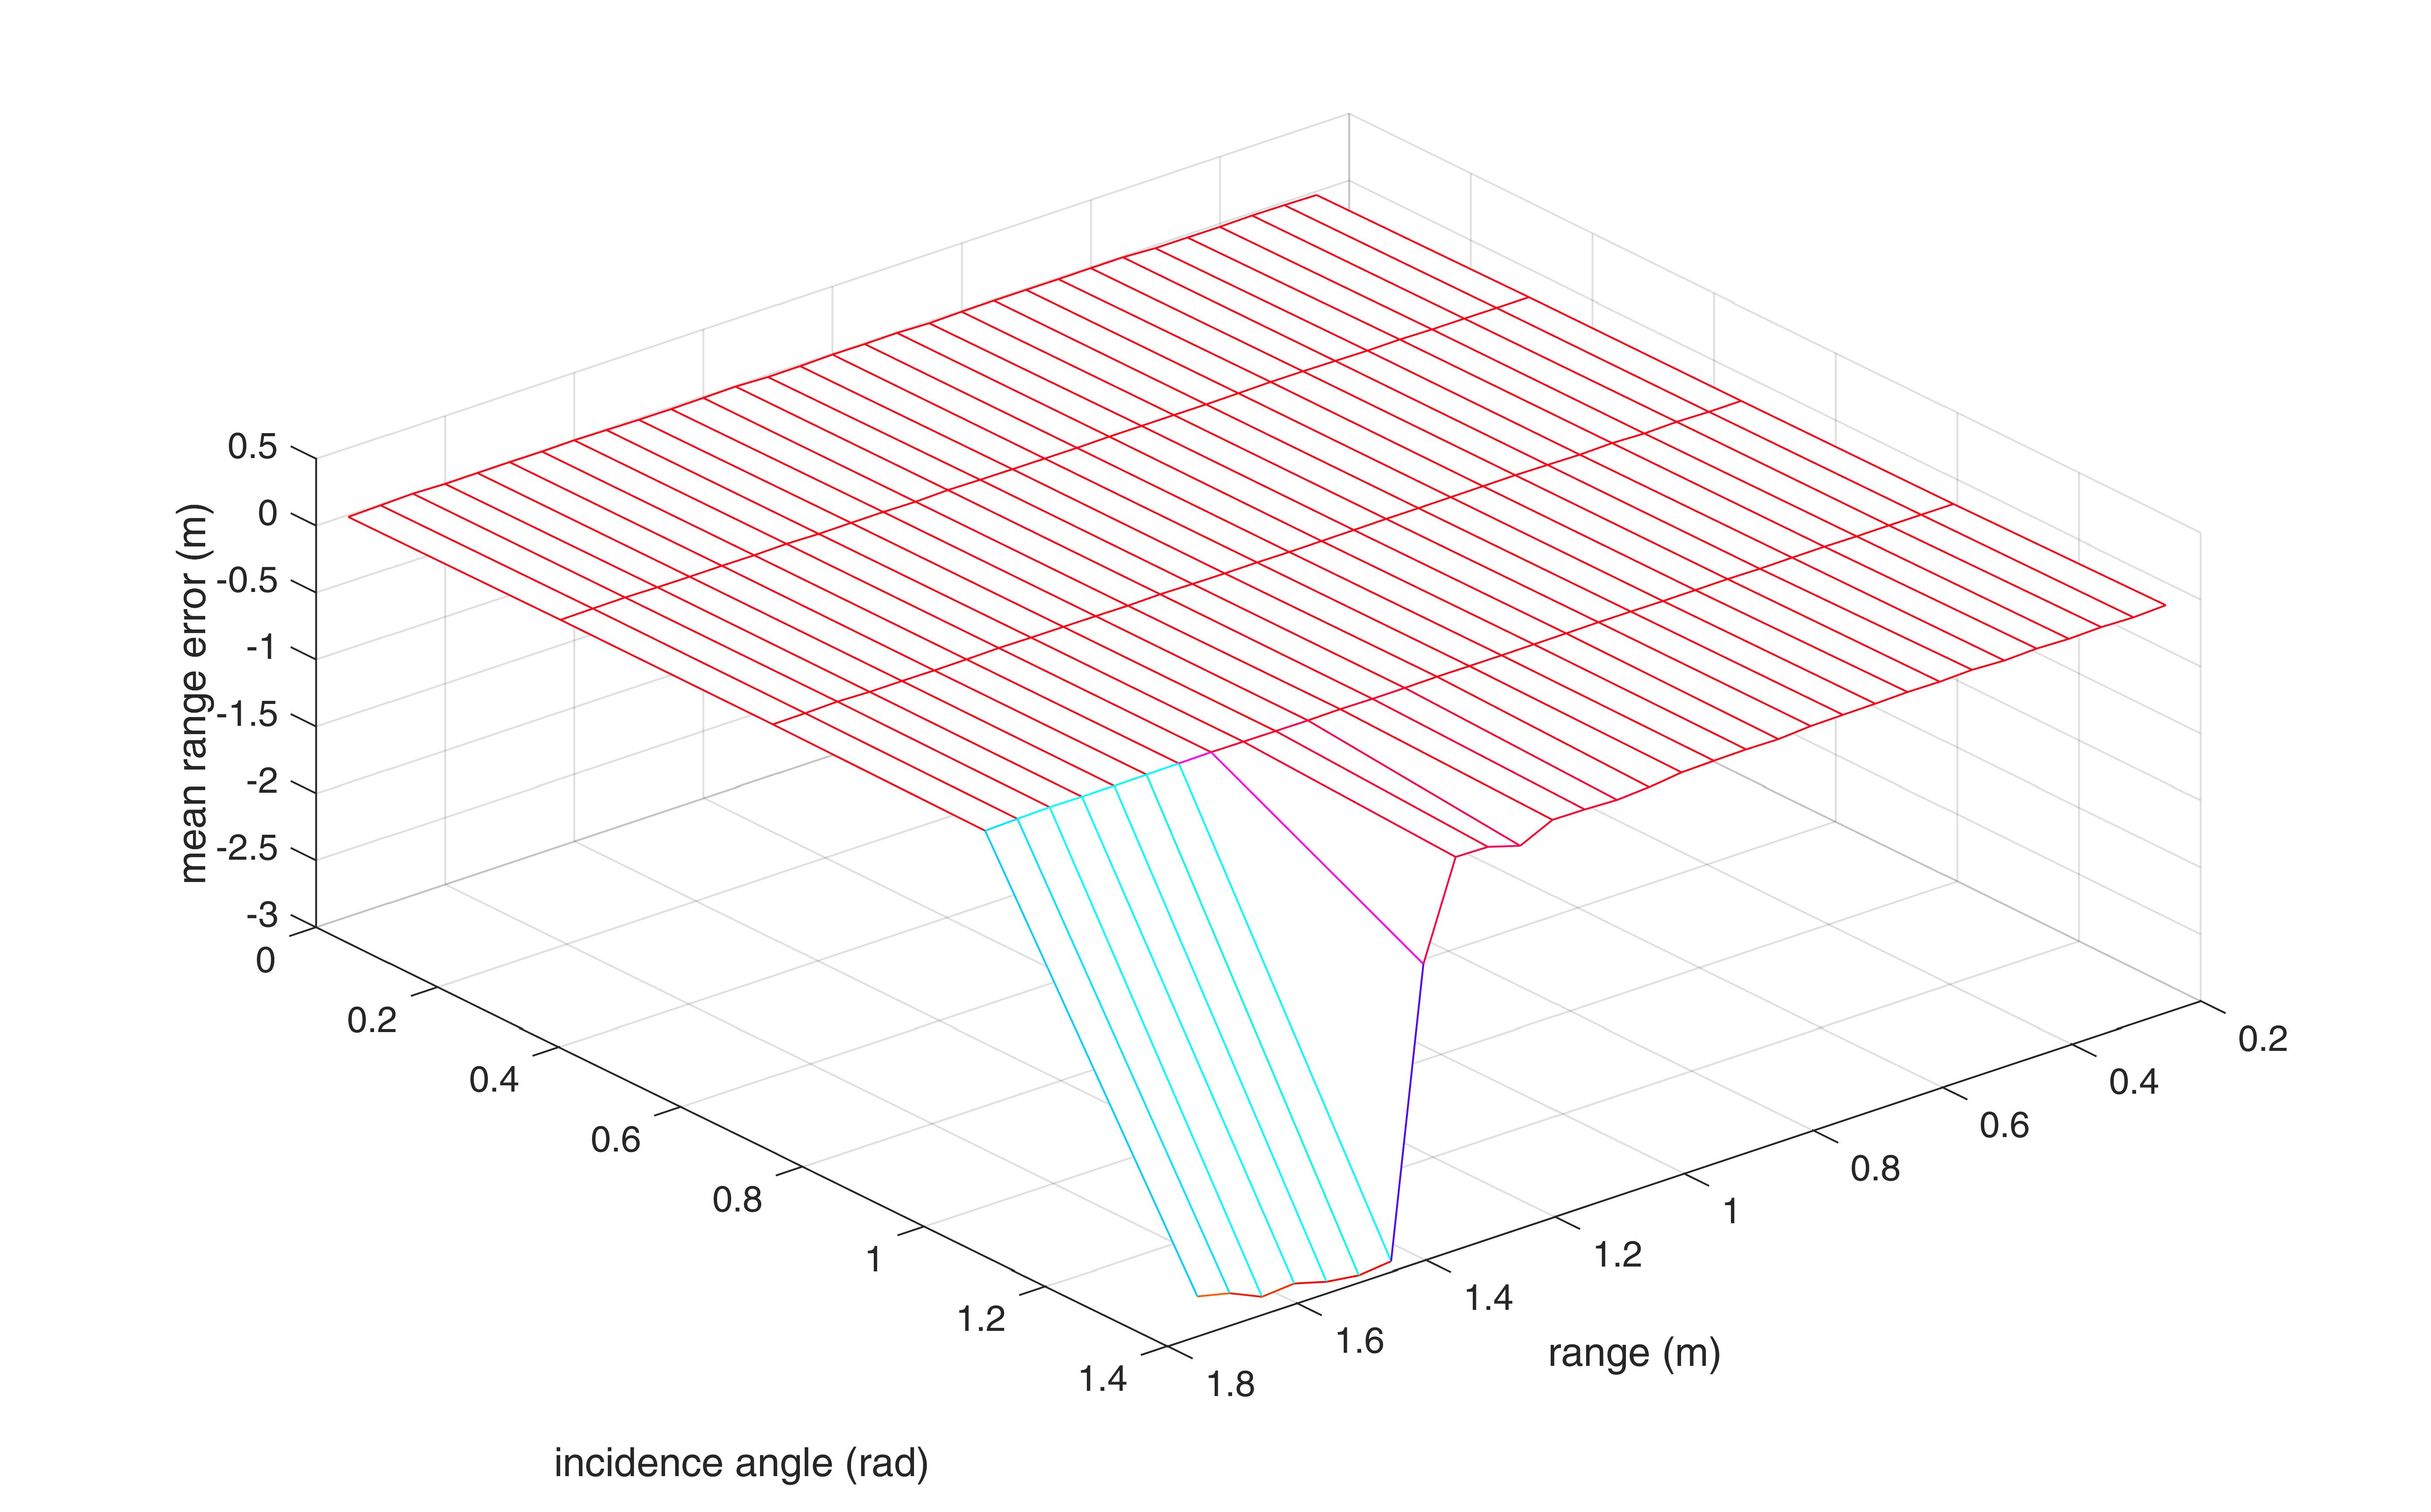
\includegraphics[width=1\textwidth,trim = 0mm 0mm 0mm 0mm,clip]{./Figures/noise_mean_range_error}\vspace*{0ex}
	  		\end{minipage}}
	  		\subfigure[\label{fig:mean_range_error_no_outliers}]{
	  		\begin{minipage}[b]{0.45\columnwidth}
    			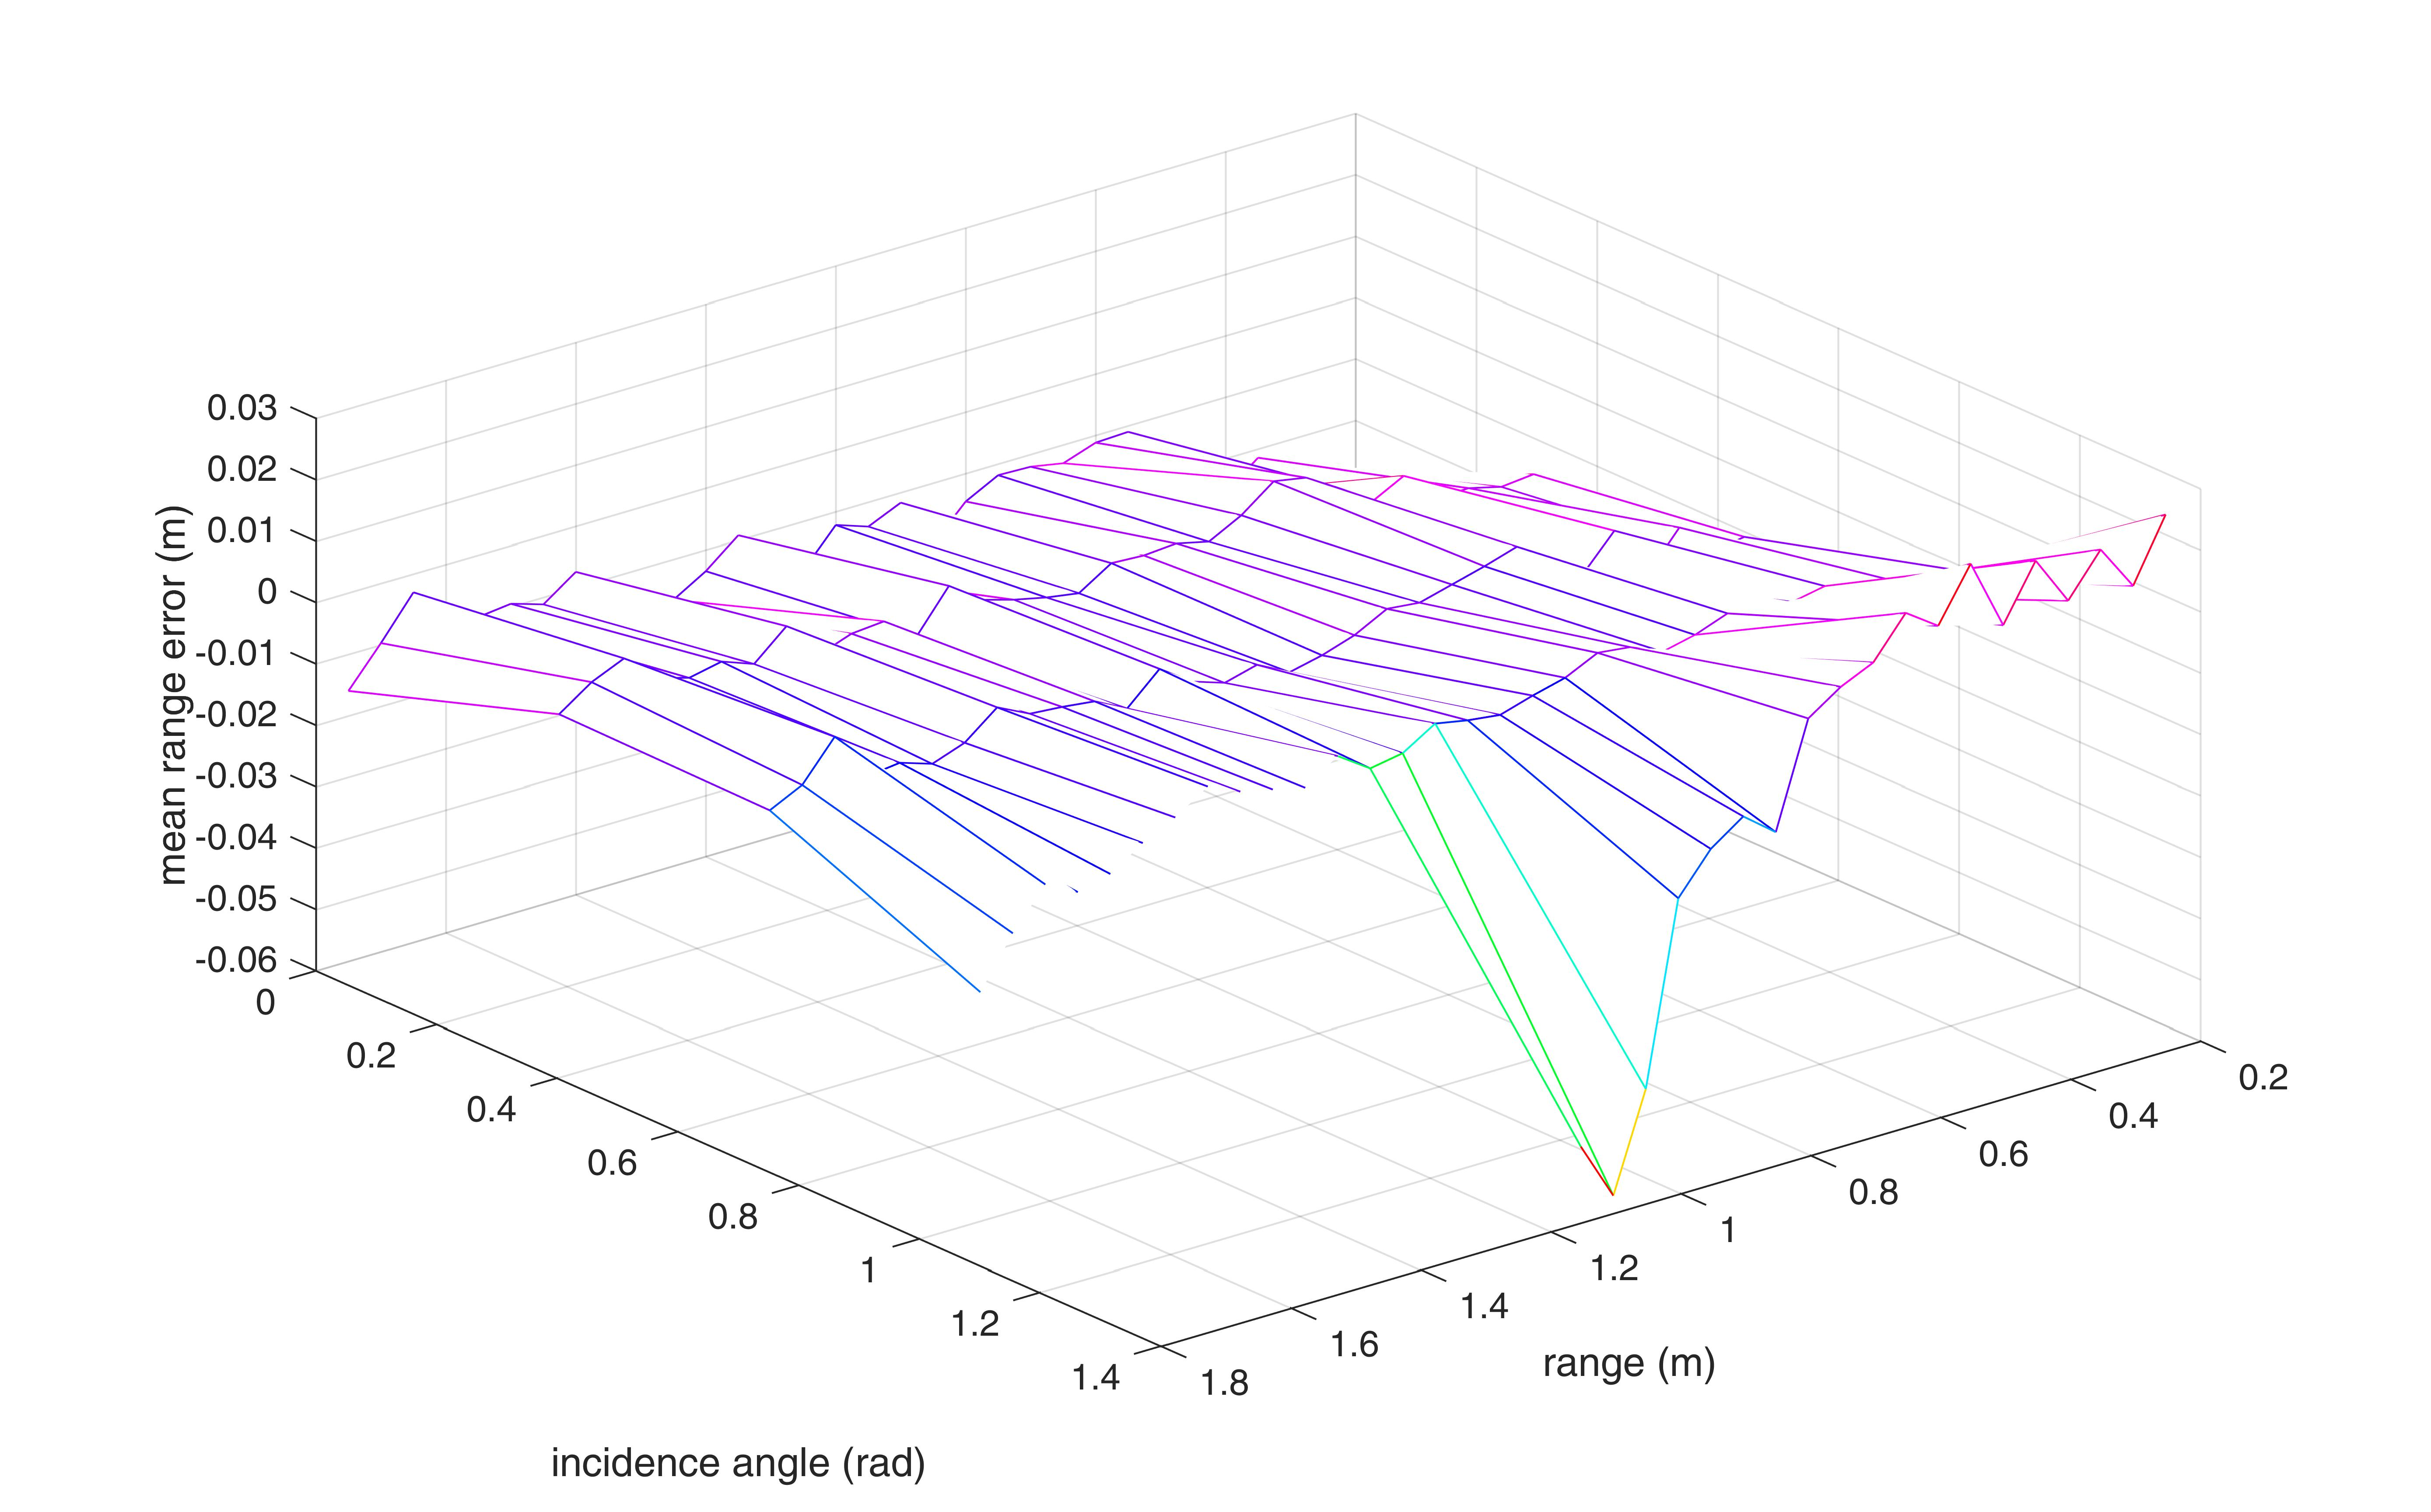
\includegraphics[width=1\textwidth,trim = 0mm 0mm 0mm 0mm,clip]{./Figures/noise_mean_range_error_removed_outliers}\vspace*{0ex}
		 \end{minipage}}
	  		\caption{mean range error vs $(r,\theta)$. (a) large error at high angles and range, (b) overall shape}
	  		\label{fig:mean_range_error}
		\end{figure}
		
		Std dev range error as function of (range,incidence angle) - Figure \ref{fig:stddev_range_error}		
		\begin{figure}
	  		\centering
	  		\subfigure[\label{fig:stddev_range_error_outliers}]{
	  		\begin{minipage}[b]{0.45\columnwidth}
    			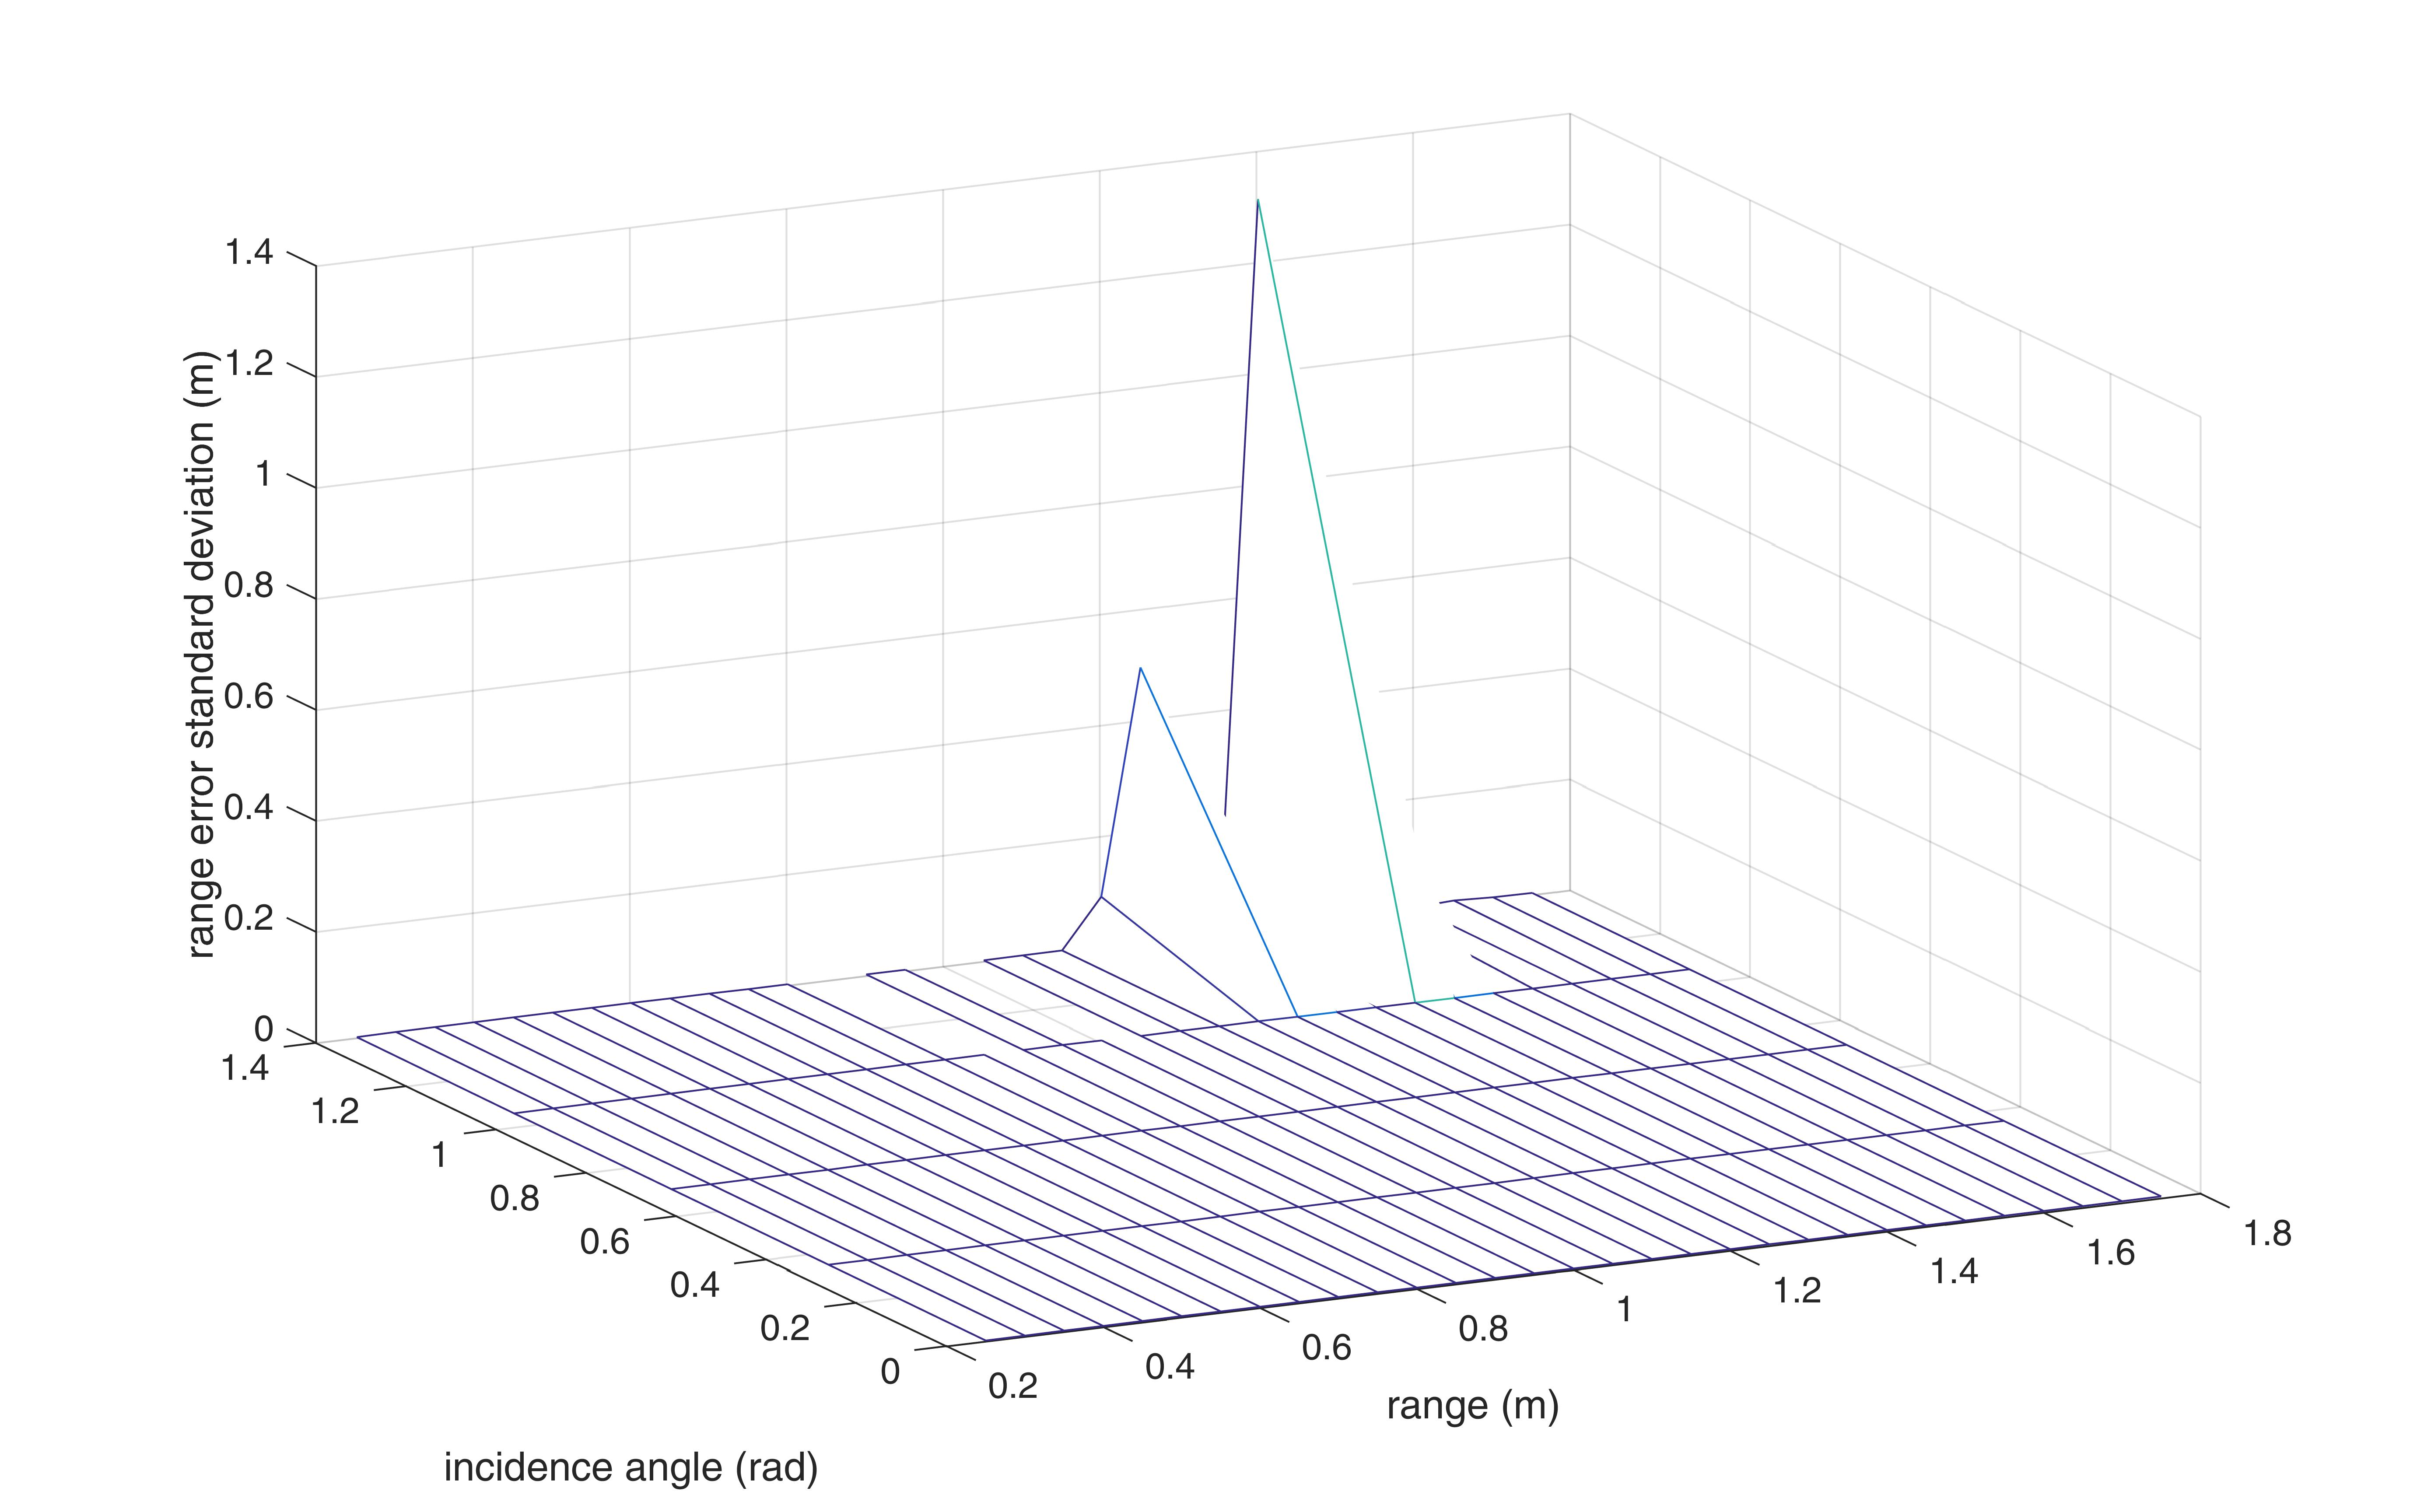
\includegraphics[width=1\textwidth,trim = 0mm 0mm 0mm 0mm,clip]{./Figures/noise_stddev_range_error}\vspace*{0ex}
	  		\end{minipage}}
	  		\subfigure[\label{fig:stddev_range_error_no_outliers}]{
	  		\begin{minipage}[b]{0.45\columnwidth}
    			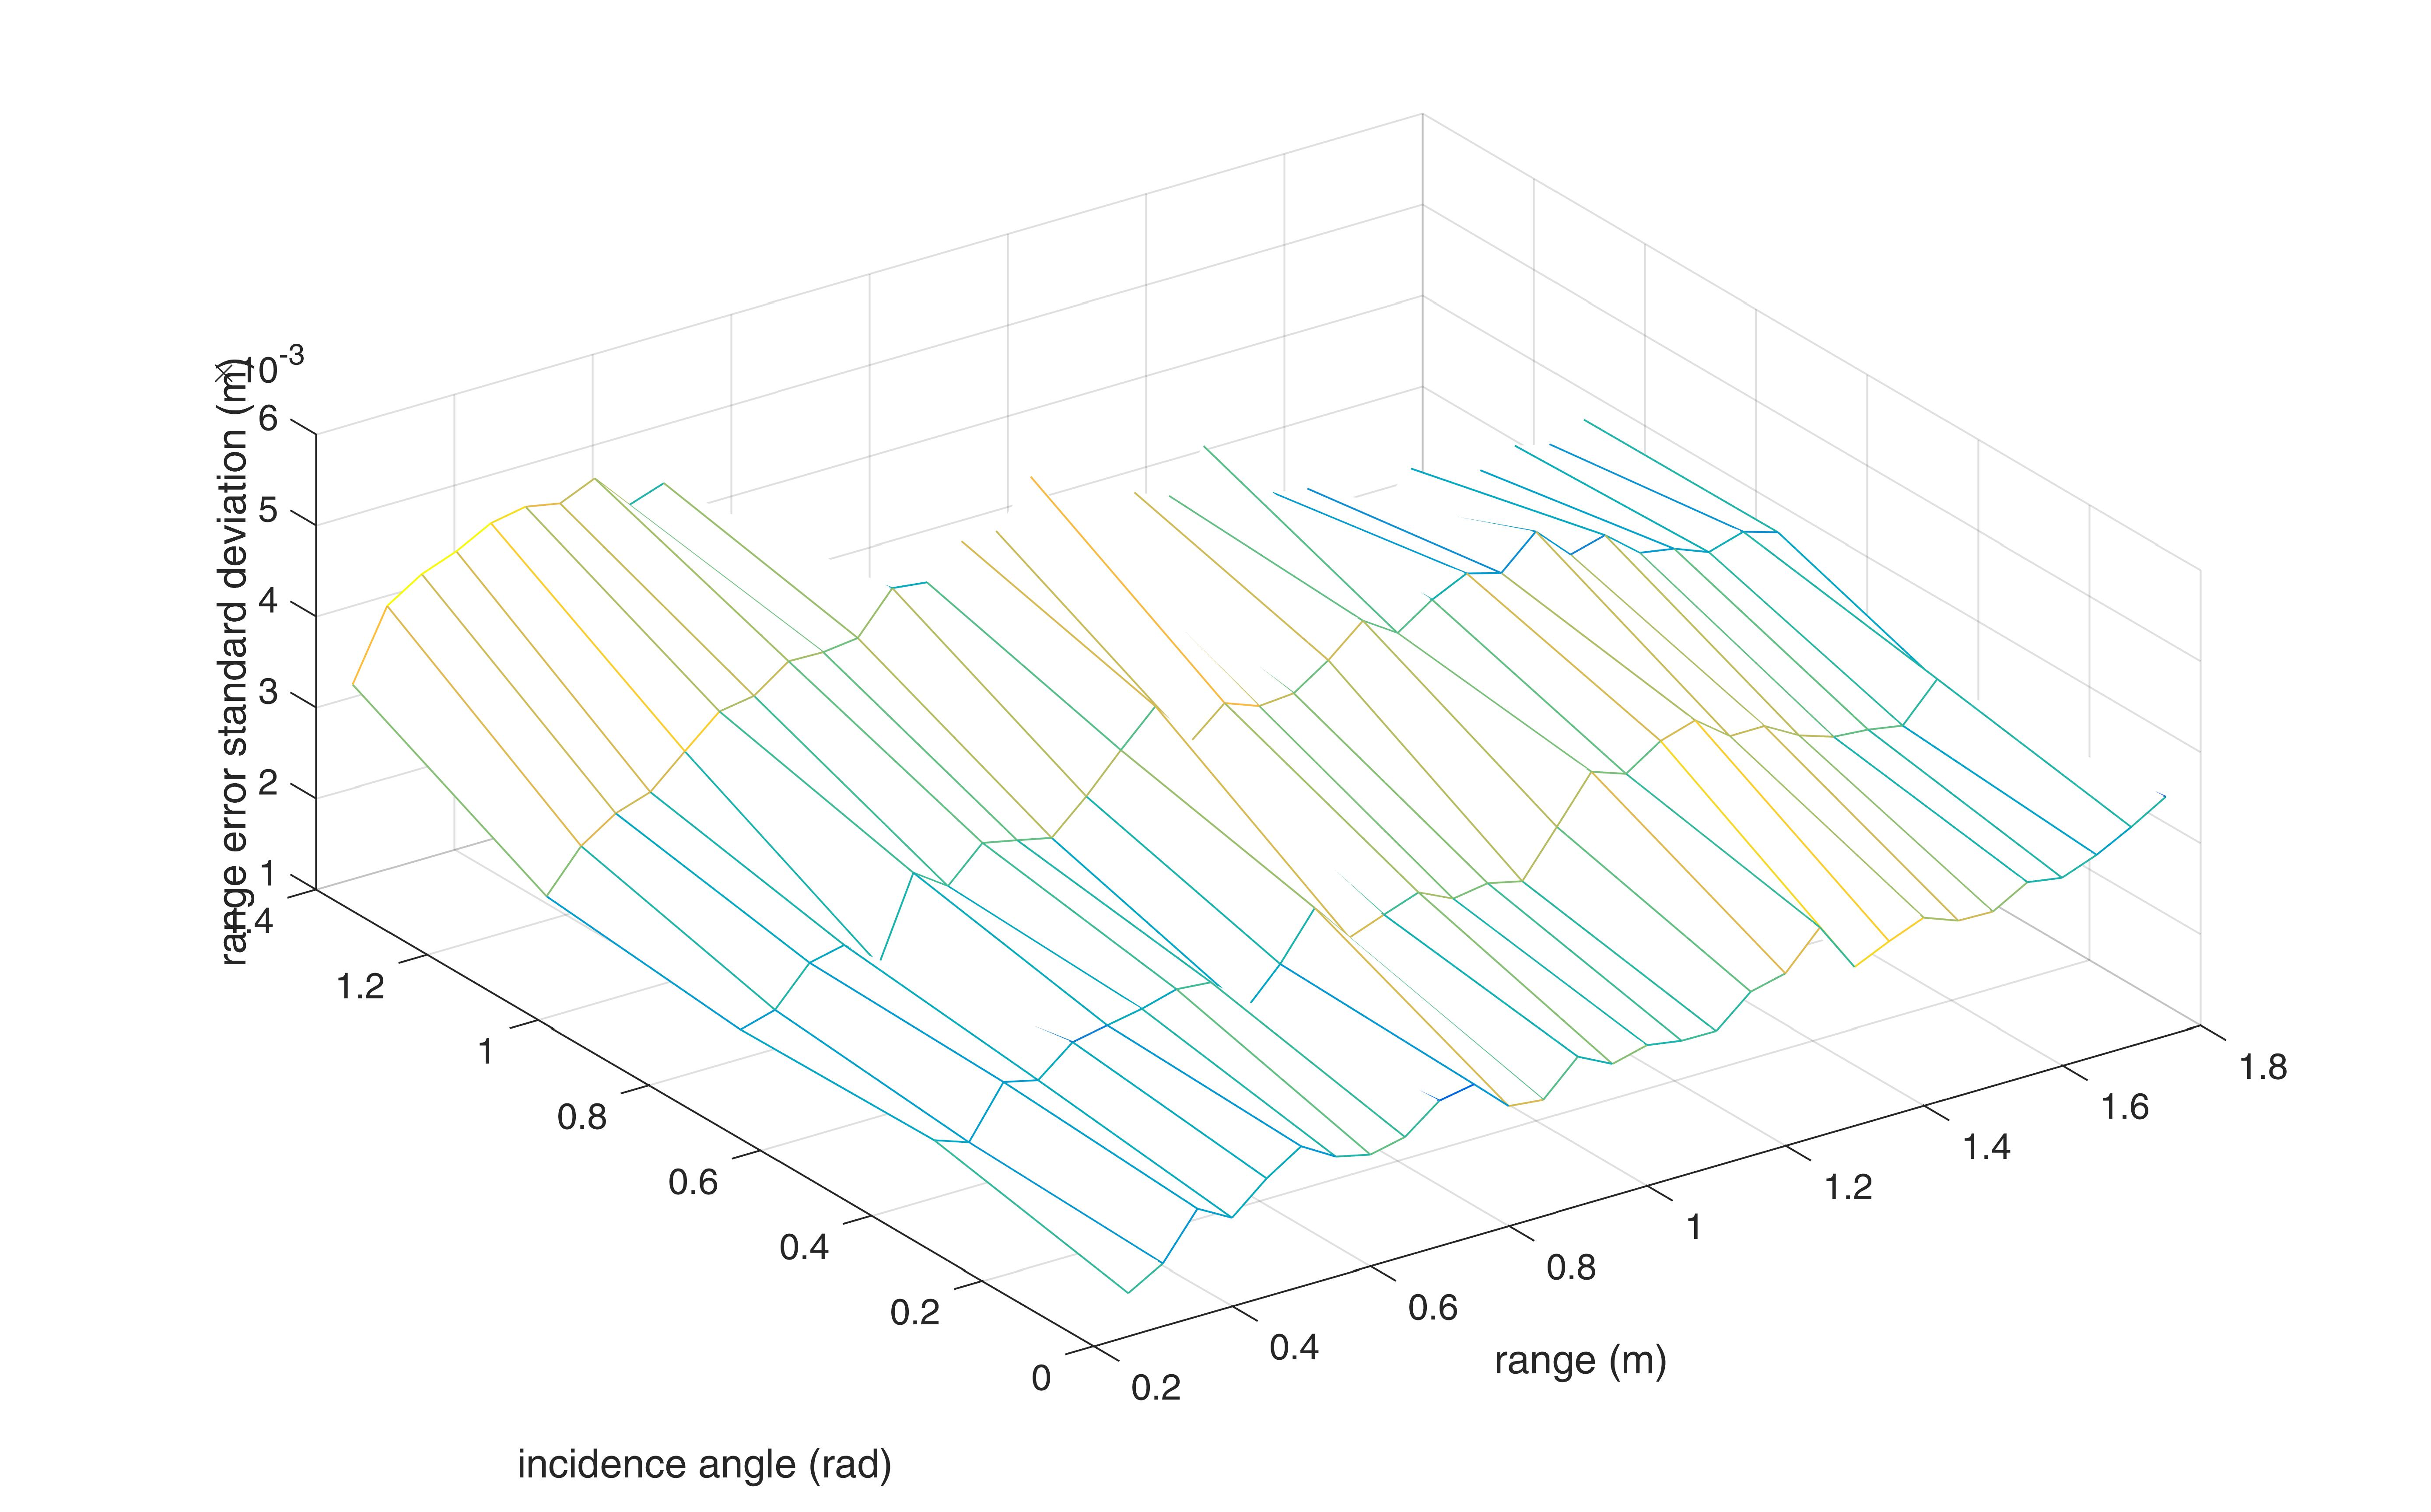
\includegraphics[width=1\textwidth,trim = 0mm 0mm 0mm 0mm,clip]{./Figures/noise_stddev_range_error_removed_outliers}\vspace*{0ex}
	 		 \end{minipage}}
	  		\caption{range error $\sigma$ vs $(r,\theta)$. (a) outliers/large std dev at high angles and range, (b) overall shape}
	  		\label{fig:stddev_range_error}
		\end{figure}
		
		Fitted 4th degree (in $x$ and $y$) polynomials to data points - Figure \ref{fig:surface_range_error}. INCLUDE FIT DATA
		\begin{figure}
	  		\centering
	  		\subfigure[\label{fig:surface_mean_range}]{
	  		\begin{minipage}[b]{0.45\columnwidth}
    			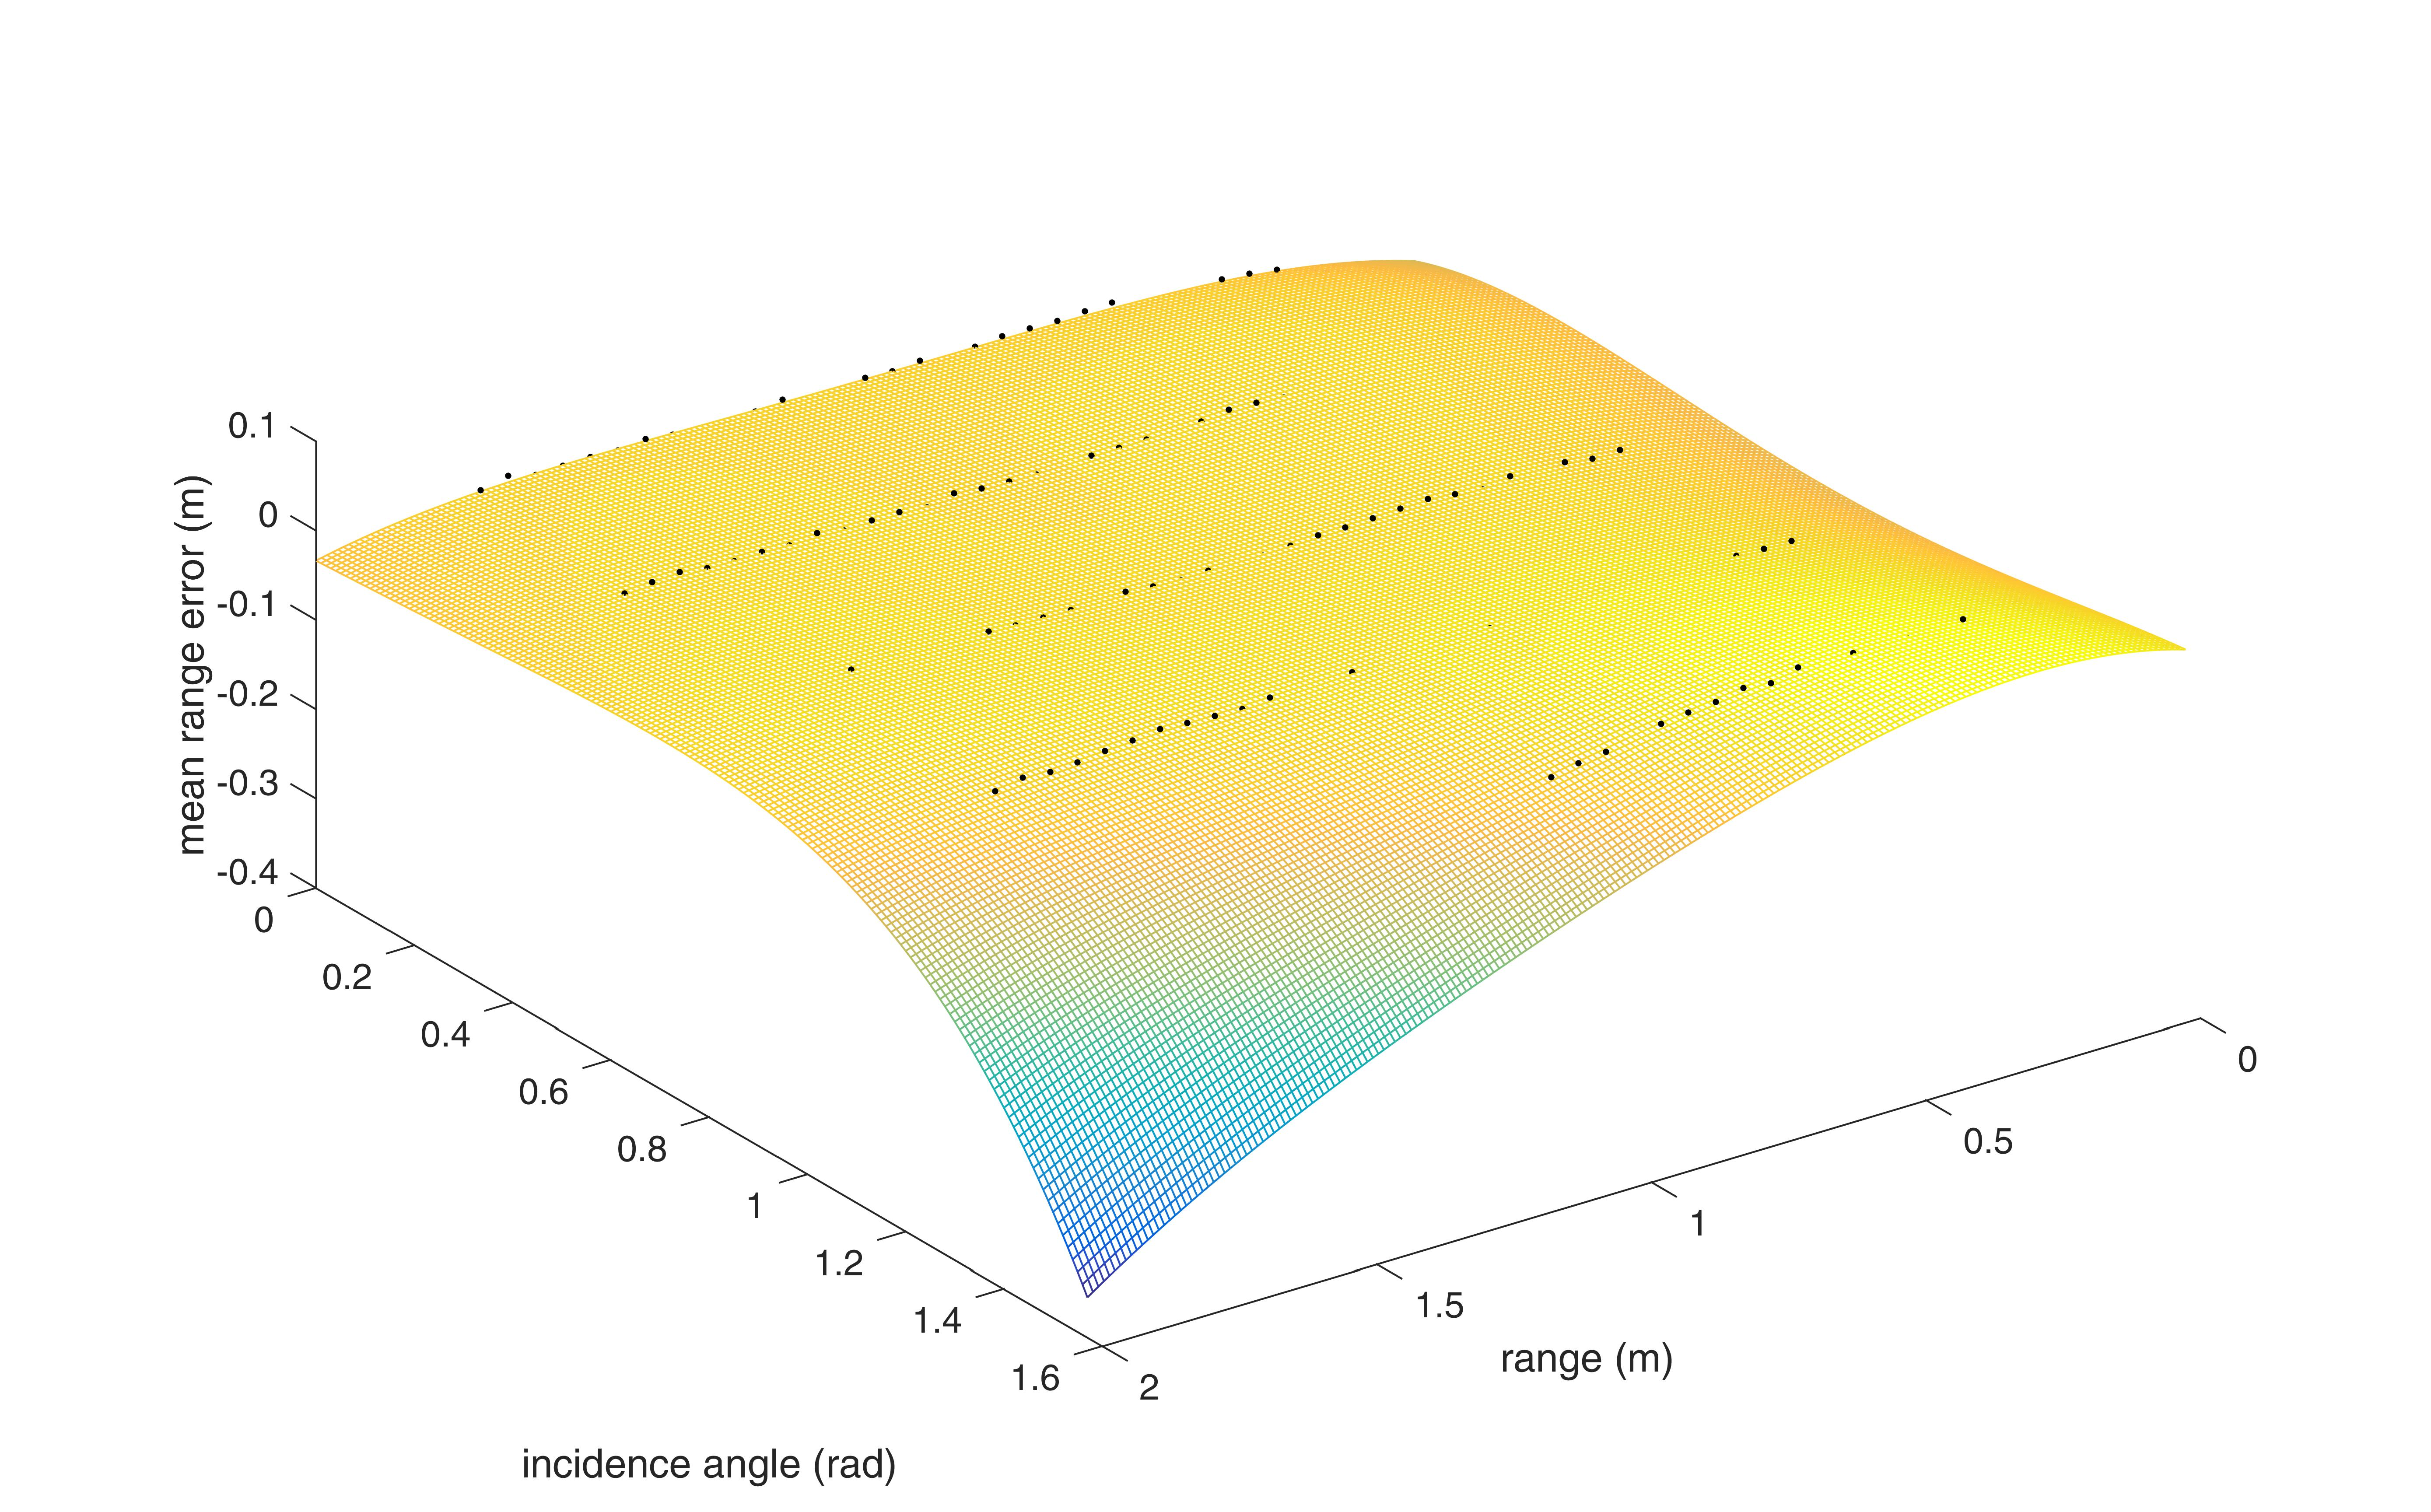
\includegraphics[width=1\textwidth,trim = 0mm 0mm 0mm 0mm,clip]{./Figures/surface_mean_range_error}\vspace*{0ex}
	  		\end{minipage}}
	  		\subfigure[\label{fig:surface_stddev_range}]{
	  		\begin{minipage}[b]{0.45\columnwidth}
    			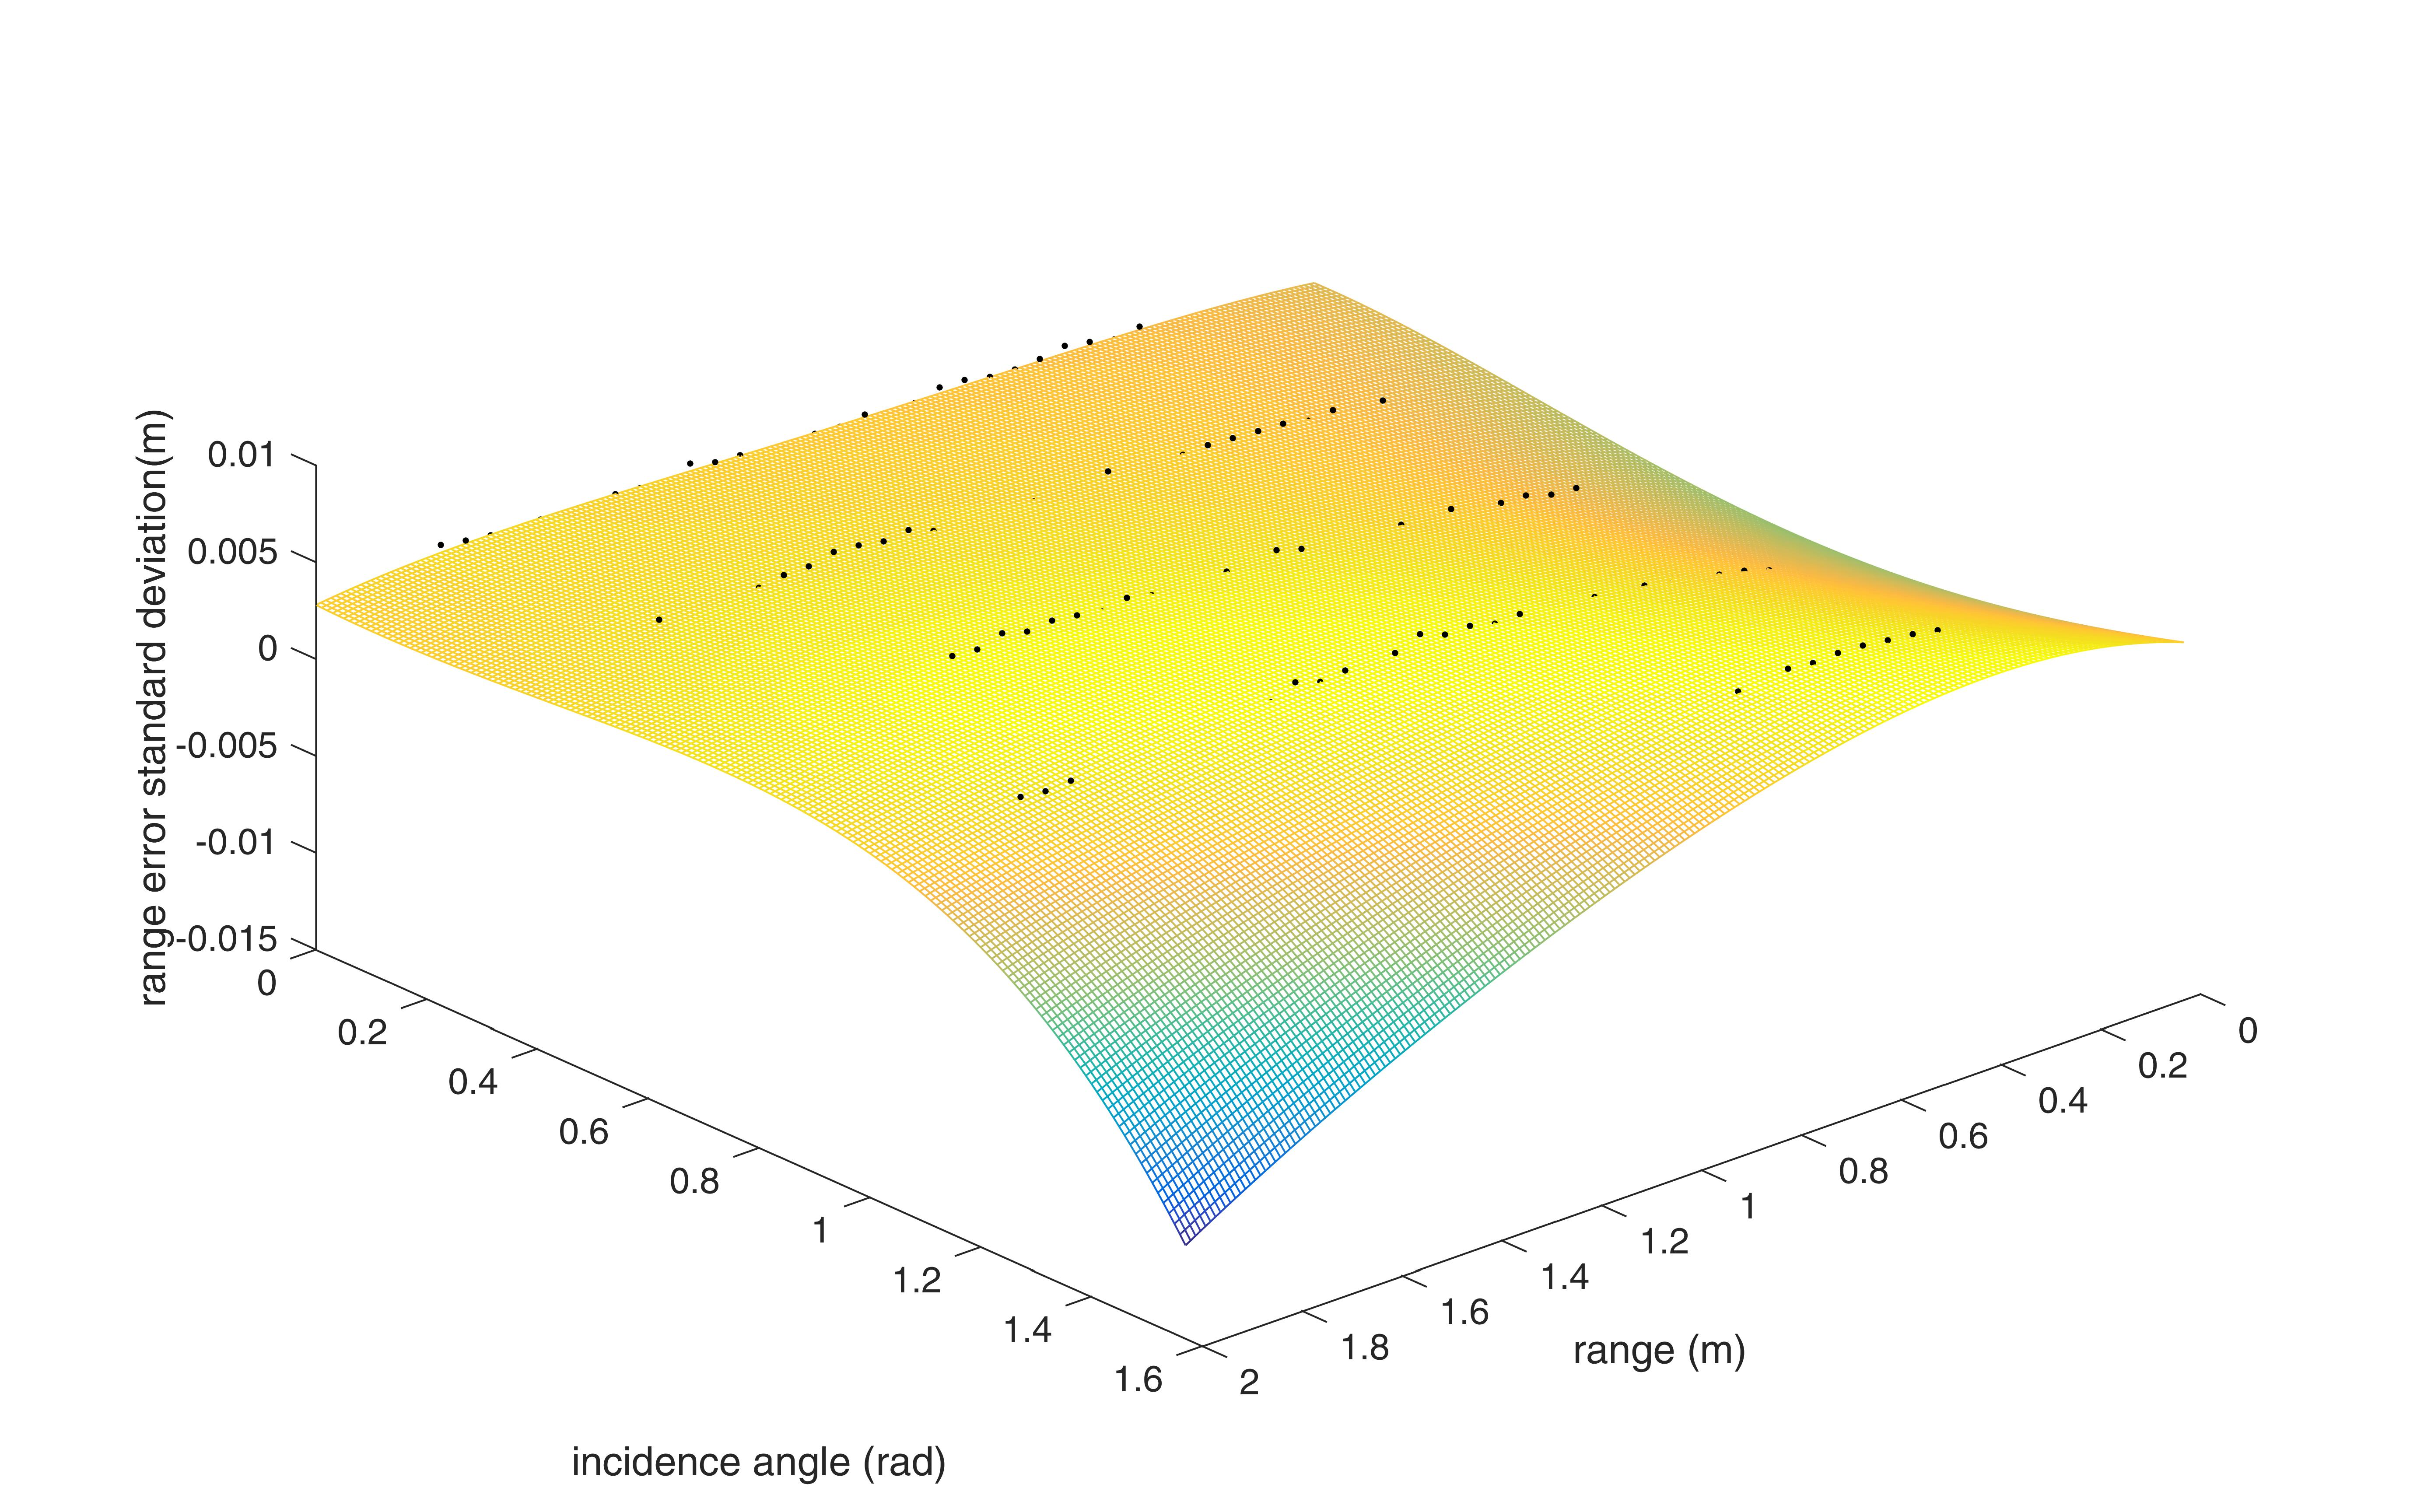
\includegraphics[width=1\textwidth,trim = 0mm 0mm 0mm 0mm,clip]{./Figures/surface_stddev_range_error}\vspace*{0ex}
		 \end{minipage}}
	  		\caption{polynomials fitted to range error mean \& standard deviation data points to model noise}
	  		\label{fig:surface_range_error}
		\end{figure}
		
		Noise Model:\\
		\begin{equation}
			\hat{r} = f_s(r,\theta,\phi(k)) = r + \mathcal{N}(\mu,\sigma)
		\end{equation}	
		
		\begin{equation}
			\begin{aligned}
				\mu = & a_{00} + a_{10}r + a_{01}\theta + a_{20}r^2 + a_{11}r\theta + a_{02}\theta^2\\
				      & + a_{30}r^3 + a_{21}r^2\theta + a_{12}r\theta^2 + a_{03}\theta^3 + a_{40}r^4 \\ 
				      & + a_{31}r^3\theta + a_{22}r^2\theta^2 + a_{13}r\theta^3 + a_{04}\theta^4
			\end{aligned}		
		\end{equation}
		\begin{equation}
			\begin{aligned}
				\sigma = & b_{00} + b_{10}r + b_{01}\theta + b_{20}r^2 + b_{11}r\theta + b_{02}\theta^2\\
			         	 & + b_{30}r^3 + b_{21}r^2\theta + b_{12}r\theta^2 + b_{03}\theta^3 + a_{40}r^4 \\ 
			         	 & + b_{31}r^3\theta + b_{22}r^2\theta^2 + b_{13}r\theta^3 + b_{04}\theta^4
			\end{aligned}
		\end{equation}
		
		*outliers ignored in model. if angle $>$ 75 deg and range $>$ 0.8m, range measurement = NaN. EXPLANATION: as angle increases, measured range becomes less than ground truth - due to beam width. part of beam hits part of object that is closer due to angle. However, as angle increases further, not enough light returns to make measurements. At high ranges and angles, measurement is not of object, but due to reflections that take much longer. Measurement ends up being near maximum range or even INF. Instead, will set as NaN - no value returned.
		
		Coefficients in tables \ref{tab:noise_a} and \ref{tab:noise_b}
		\begin{table}[h!]
  \centering
  \caption{$a_{ij}$ coefficients}
  \label{tab:noise_a}
  \begin{tabular}{c| c c c c c}
     	  & $j_0$ 	 & $j_1$   & $j_2$ 	 & $j_3$   & $j_4$ \\
    \hline
   	$i_0$ & -0.06529 & 0.2126  & -0.533	 & 0.4629  & -0.1223 \\
   	$i_1$ & 0.2024   & -0.1906 & 0.4006	 & -0.1791 & 0 \\
   	$i_2$ & -0.3074  & 0.0228  & -0.0716 & 0 	   & 0 \\
   	$i_3$ & 0.2053   & 0.01455 & 0 		 & 0 	   & 0 \\
   	$i_4$ & -0.04912 & 0 	   & 0 		 & 0 	   & 0 \\
  \end{tabular}
\end{table}



		\begin{table}[h!]
  \centering
  \caption{$b_{ij}$ coefficients}
  \label{tab:noise_b}
  \begin{tabular}{c| c c c c c}
		  & $j_0$ 	  & $j_1$    & $j_2$ 	  & $j_3$	  & $j_4$ \\
	\hline
	$i_0$ & 0.001242  & 0.2126	 & -0.01128	  & 0.01162	  & -0.002746 \\
	$i_1$ & 0.00352   & 0.006146 & 0.01021	  & -0.007316 & 0 \\
	$i_2$ & -0.005138 & -0.00626 & -0.0005068 & 0 		  & 0 \\
	$i_3$ & 0.004067  & 0.001337 & 0 		  & 0 		  & 0 \\
	$i_4$ & -0.001092 & 0 		 & 0 		  & 0 		  & 0 \\
  \end{tabular}
\end{table}





		\textbf{Surface noise:}
		random walk model\\
		have observed error mostly independent of range and angle - seems to be some compensation performed by sensor to get straight lines - range across smooth surfaces that should be appear as straight lines varies regularly.
		Could be surface properties of objects, though error is larger than expected in this case.
		Profile of error sinusoidal (regular-ish peaks and valleys), peaks = 5mm deep \& 50mm wide approximately
		
		add random walk to each scan
		\begin{equation}
			error = a\sum_{n = 1}^{n_{Steps}}-1 + 2\:\left \lfloor{\mathcal{R}}\right \rfloor 
		\end{equation} 
		where $\mathcal{R}$ is a random variable following a uniform distribution on [0,1]. Chose step size of $a = 0.0005m$
		Doesn't work too well over long surfaces (~1m) - can get too large sometimes, but fits measured data for small objects like cube
		
		Figure \ref{fig:surface_noise}: comparison of simulated \& measured surface noise:
		\textbf{ERROR BARS INSTEAD OF DOTS}. MENTION THAT IT IS FLIPPED, COULD BE OTHER WAY. DUE TO RANDOM WALK.
		\begin{figure}
	  		\centering
	  		\subfigure[\label{fig:measured_surface_noise}]{
	  		\begin{minipage}[b]{0.45\columnwidth}
    			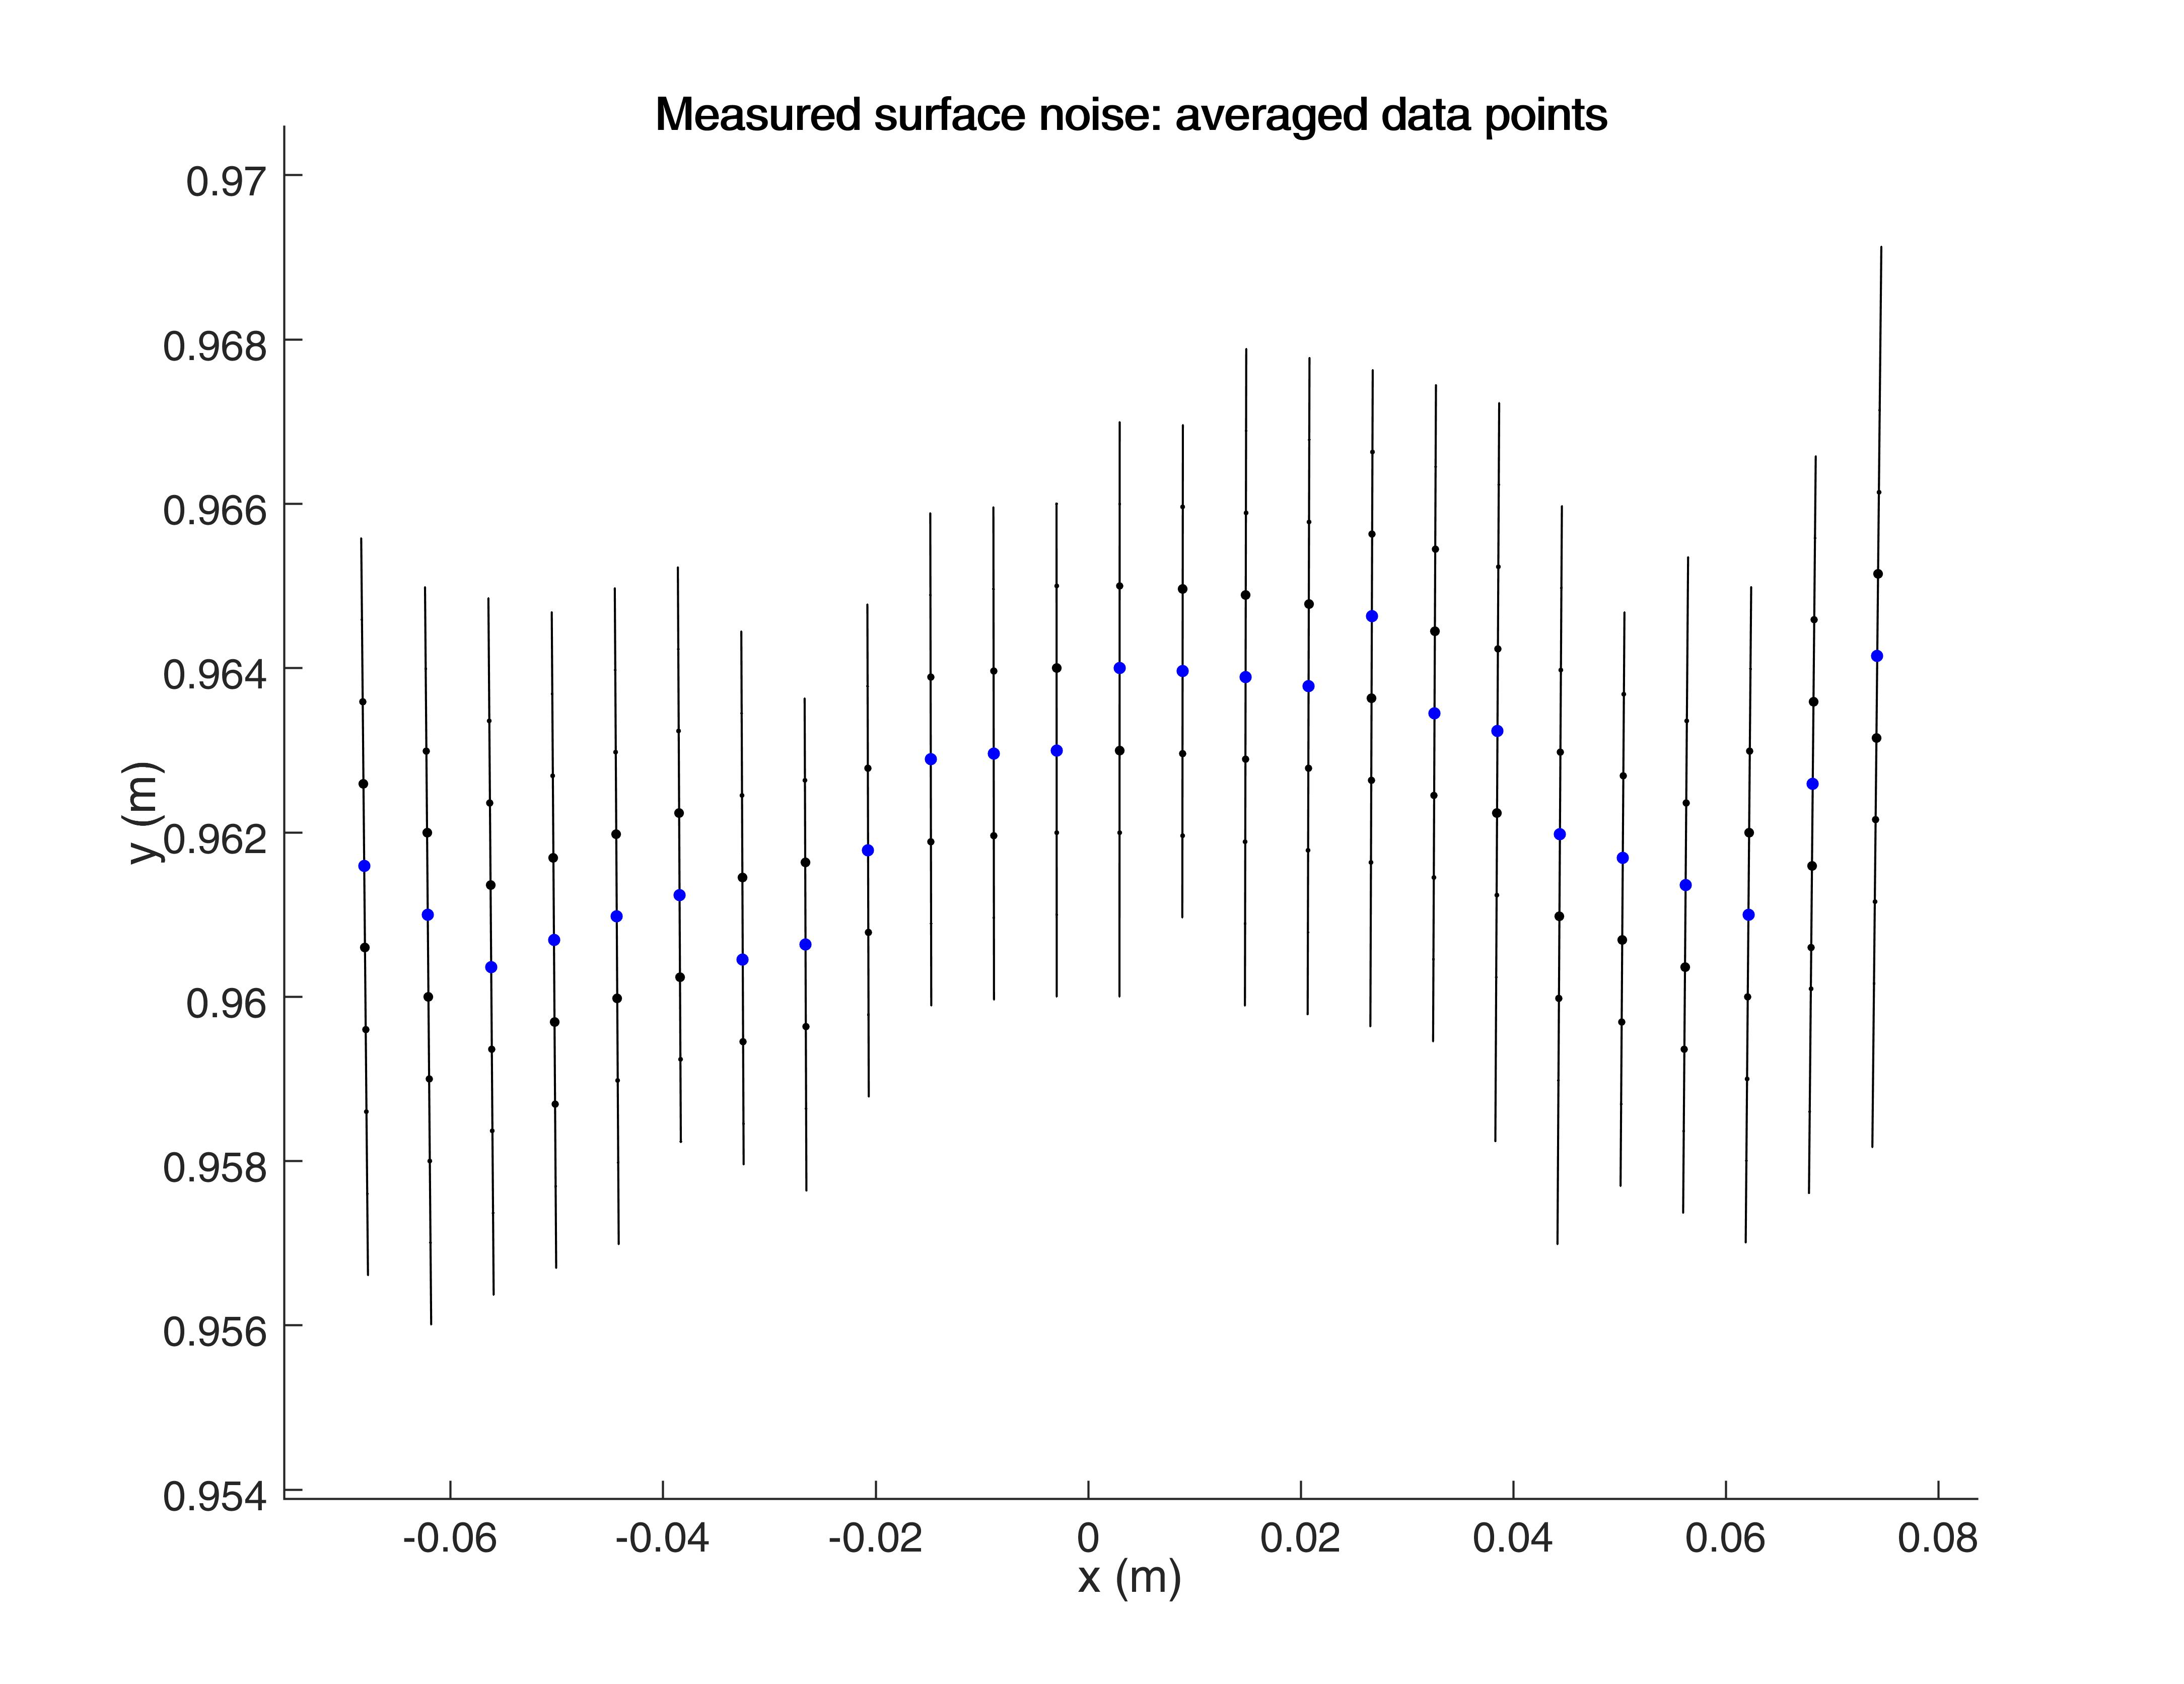
\includegraphics[width=1\textwidth,trim = 0mm 0mm 0mm 0mm,clip]{./Figures/measured_surface_noise}\vspace*{0ex}
	  		\end{minipage}}
	  		\subfigure[\label{fig:simulated_surface_noise}]{
	  		\begin{minipage}[b]{0.45\columnwidth}
    			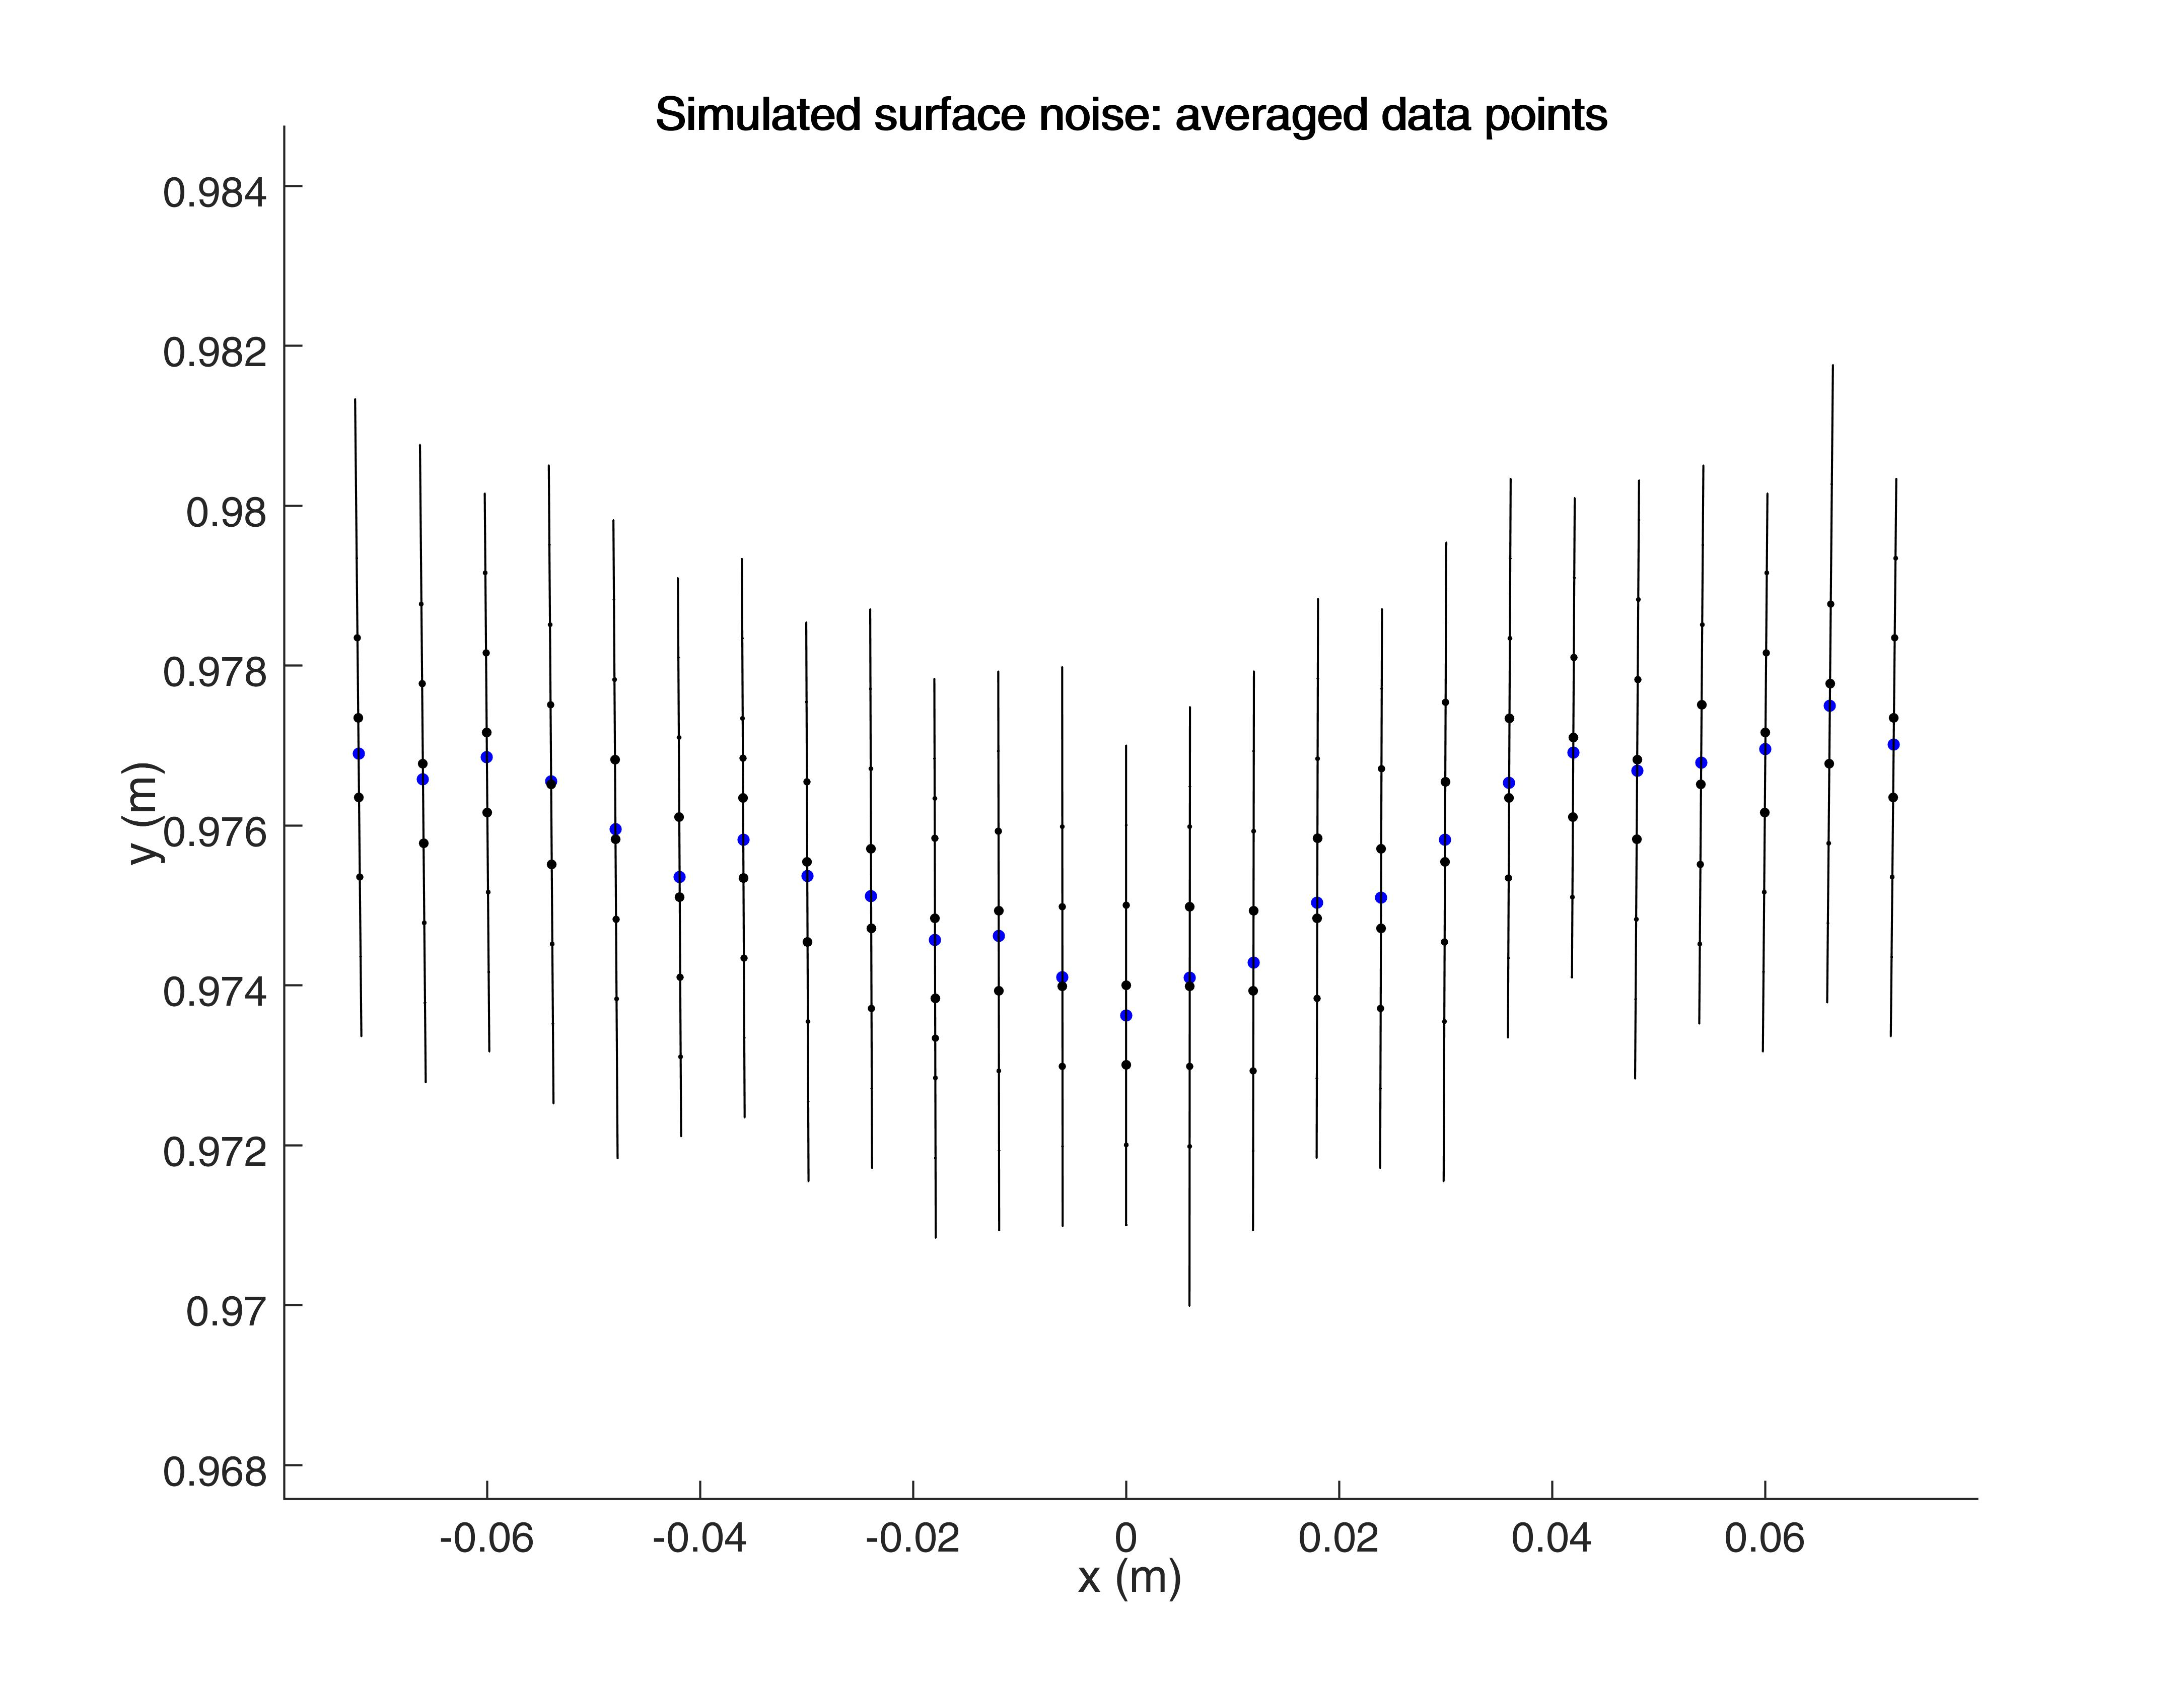
\includegraphics[width=1\textwidth,trim = 0mm 0mm 0mm 0mm,clip]{./Figures/simulated_surface_noise}\vspace*{0ex}
 			\end{minipage}}
	  		\caption{Comparision of (a) measured and (b) simulated surface noise}
	  		\label{fig:surface_noise}
		\end{figure}

\section{Testing Data Collection} \label{testingdata}
	\subsection{Setup}
		physical setup - \ref{experimental_data} PICS IN APPENDIX\\
		Real world, less than ideal conditions.
		Sensor:\\
		Hokuyo UBG-04LX-F01 - 2D scanning laser range-finder. Measures range\\
		
		Robot arm: \\
		Kinova Jaco - can program to move with and record pose
		
		Target object: \\
		$0.1 \times 0.1$ m MDF cube, spray painted matte white
		
		configurations/motions: \\
			-stationary\\
			-rotating\\
			-translating\\					
		arm forward kinematics $\rightarrow$ cube pose\\
		estimate sensor angle with horizontal with wall calibration data		
		
	\subsection{Results}
		still need to calibrate data.
		However, prediction is observer wont work. First, neither range or continuity assumptions will hold - gripper hold cube will mess with things. Lots of noise.
		Likely will need an infinite dimensional observer, estimate entire depth field. Need symmetry to get robust convergence.
		Still, data is available for future research.

